\documentclass[oneside]{book}
\usepackage{url,verbatim,fancyvrb}
\usepackage{pifont}
\usepackage[utf8]{inputenc}
\usepackage[pdftex]{graphicx}
\usepackage[authoryear]{natbib}
\usepackage{gretl}
\usepackage[letterpaper,body={6.3in,9.15in},top=.8in,left=1.1in]{geometry}
\usepackage[pdftex,hyperfootnotes=false]{hyperref}
\usepackage{dcolumn,amsmath,bm}

\newcommand{\ttusage}[1]{\textit{example}: \quad \texttt{#1}}
\newcommand{\vbusage}[0]{\textit{example}: \quad}

\setcounter{secnumdepth}{2}

\bibliographystyle{gretl}

%% \pdfimageresolution=120
\hypersetup{pdftitle={Gretl Function Package Guide},
            pdfsubject={Using and writing gretl function packages},
            pdfauthor={Allin Cottrell and Riccardo (Jack) Lucchetti},
            colorlinks=true,
            linkcolor=blue,
            urlcolor=red,
            citecolor=steel,
            bookmarks=true,
            bookmarksnumbered=true,
            plainpages=false
}

\begin{document}

\VerbatimFootnotes

\setlength{\parindent}{0pt}
\setlength{\parskip}{1ex}
\setcounter{tocdepth}{1}

%% titlepage

\thispagestyle{empty}

\begin{center}
\pdfbookmark[1]{Gretl Function Package Guide}{titlepage}

\gtitle{Gretl Function Package Guide}

{\large \sffamily
Allin Cottrell\\
Department of Economics\\
Wake Forest University\\

\vspace{20pt}
Riccardo (Jack) Lucchetti\\
Dipartimento di Scienze Economiche e Sociali\\
Università Politecnica delle Marche\\

\vspace{20pt}
\input date
}

\end{center}
\clearpage

%% end titlepage, start license page

\thispagestyle{empty}

\pdfbookmark[1]{License}{license}

\vspace*{2in}

Permission is granted to copy, distribute and/or modify this document
under the terms of the \emph{GNU Free Documentation License}, Version
1.1 or any later version published by the Free Software Foundation
(see \url{http://www.gnu.org/licenses/fdl.html}).

\cleardoublepage

%% end license page, start table of contents
\pdfbookmark[1]{Table of contents}{contents}

\pagenumbering{roman}
\pagestyle{headings}

\tableofcontents

\clearpage
\pagenumbering{arabic}
%\setcounter{chapter}{-1}

\chapter{Introduction}
\label{chap:intro}

\section{The purpose of function packages}
\label{sec:purpose}

The primary purpose of gretl function packages is to add estimators,
hypothesis tests or other analytical procedures to gretl's repertoire
of built-in procedures. While function packages may also be used for
other purposes (e.g.\ pedagogy, replication exercises), those made
available via the gretl server are expected to extend gretl's
functionality in non-trivial ways.\footnote{For an extended discussion
  of the rationale for such packages see ``Extending gretl: addons and
  bundles'' \citep{addons-bundles}. Note, however, that the
  distinction between regular packages and ``addons'' in that document
  has become somewhat blurred, as regular packages have gradually
  acquired many of the rights and responsibilities previously confined
  to official gretl ``addons''. On the rights side, regular packages
  are now able to hook into the gretl GUI; on the responsibilities
  side, contributed packages are now subject to a degree of vetting
  before they can appear in the public download area on the gretl
  server.}

\section{The form of function packages}
\label{sec:pkgform}

The core component of a gretl function package---in simpler cases,
the sole component---is a \textsf{gfn} file. This is an XML file
conforming to the Document Type Definition \texttt{gretlfunc.dtd},
which is supplied in the gretl distribution; the latest version can
always be found online.\footnote{See
  \url{http://sourceforge.net/p/gretl/git/ci/master/tree/share/functions/gretlfunc.dtd}.}
Such files contain
\begin{itemize}
\item the hansl code for at least one function;
\item various items of metadata (author, version, date, etc.);
\item help text for the function(s), or a pointer to help in
  PDF format; and
\item a sample script that illustrates a call to the packaged
  function(s).
\end{itemize}

While it is possible in principle to create and edit a \textsf{gfn}
file ``manually'', using a suitable text editor, this is not
recommended. Gretl provides tools (both command-line and GUI) to create
and maintain package files, so that authors are not required to
mess with raw XML.

We will refer to packages that consist of a gfn file alone as ``simple
packages'' (the included hansl code may not be particularly simple,
but the structure is simple).

The alternative to a simple package we will call a ``zip package''.
Such packages take the form of a \textsf{PKZIP} archive containing a
\texttt{gfn} file along with other materials, which may include PDF
documentation (in place of plain text help), data needed by the
package for internal use (for example, tables of critical values for
some test statistic), and/or extra data files or scripts intended to
supplement the required sample script. Zip packages can be built using
command-line tools or with the help of the gretl GUI.

One point to note about zip packages is that the \textsf{PKZIP}
wrapper is actually just a storage and transport format. When such a
package is installed, it is unpacked in a suitable location. Further
details on this package format can be found in
chapter~\ref{chap:zipfile}.

\section{Using this document}

Chapter~\ref{chap:users} gives an account of function packages from
the user's point of view. Even those who are familiar with packages
might want to take a look, since there are some finer points that
might not be immediately evident. Moreover, there have been several
changes and enhancements in recent gretl versions.

Chapter~\ref{chap:authors} takes the author's point of view, giving a
walk-through of the means of creating, refining and publishing
function packages, both via the command-line and via the GUI.

Chapters~\ref{chap:specfile} and \ref{chap:zipfile} provide reference
material on the details of package specification and structure, along
with some tips on usage.

%%%%%%%%%%%%%%%% chapter break %%%%%%%%%%%%%%%%%

\chapter{For package users}
\label{chap:users}

\section{The two package browsers}
\label{sec:browsers}

Since we'll be referring to the ``browsers'' for function packages
quite a lot in the following, let us be clear up front about the two
package browser windows in gretl and how they are accessed.

One of these windows shows the packages installed on your own
computer. To open it, either select the menu item ``File, Function
packages, On local machine'' or use the short-cut button labeled
``$fx$'' on the toolbar at the foot of the main gretl
window. With a new installation of gretl there will not be much to see
in this window at first.

The other browser shows all the packages available from the gretl
server. It can be opened via the menu item ``File, Function packages,
On server.'' The same listing can be accessed via a web
interface,\footnote{See
  \url{http://gretl.sourceforge.net/cgi-bin/gretldata.cgi?opt=SHOW_FUNCS}.}
but for most purposes it will probably be more convenient to work from
within gretl.

The two browsers are interconnected: from the ``local machine'' window
you can open the ``on server'' one by clicking on the Network button
in the toolbar (tooltip, ``Look on server''), while from the latter
you can open or focus the ``local machine'' window by clicking the
Home button (tooltip, ``Local machine''). They are also connected via
drag-and-drop: one way of installing a package from the server is by
selecting it in the server window and dragging it onto the local one.

When we use the term ``package browser'' below we will generally mean
the local window; we'll add the qualification ``on server'' when we're
talking about the other one. For screenshots of both browsers see
Section~\ref{sec:gui-install} below.

That said, let's move on to the business of getting hold of a function
package of interest.

\section{Acquiring a package}
\label{sec:acquire}

We'll focus here on packages available from the gretl server. These
have passed a checking procedure on the part of the gretl development
team, designed to ensure that they are usable with the current version
of gretl. This does not mean, however, that they are guaranteed to be
bug-free, or to deliver accurate results; those responsibilities rest
on the shoulders of the package authors.

Some authors may choose to make their packages available via other
means. In that case, once the user has the package file available,
either as a \textsf{gfn} file or a \textsf{zip} file (see
Section~\ref{sec:pkgform}), the package can be installed using
the instructions below (Section \ref{sec:cli-install}).

\subsection{Installing a package via the GUI}
\label{sec:gui-install}

We'll use as an example Ignacio D\'iaz-Emparanza's \textsf{GHegy}
package.  Suppose you've read Ignacio's excellent paper on seasonal
unit-root tests \citep{Ignacio-HEGY} and you'd like to use his
results. You were told a gretl package is available. Here's what you
do. (We assume you have an Internet connection.)

Open gretl, and select ``File, Function packages, On server''. Since
the package deals with seasonal unit roots, you'll probably want to
look for the word ``seasonal''. After typing \texttt{seasonal} in the
top-right search box and hitting the \textsf{Enter} key a few times,
you find what looks like it (Figure~\ref{fig:ghegy-lst}).

\begin{figure}[htbp]
\begin{center}
  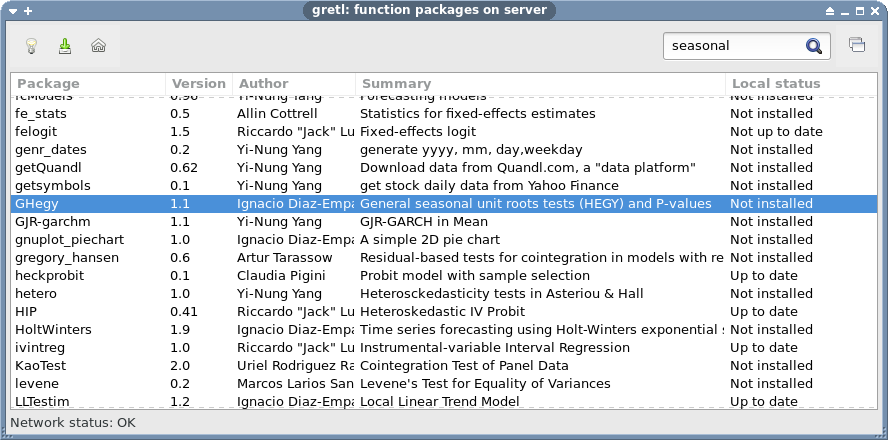
\includegraphics[scale=0.5]{figures/ghegy-lst.png}
\end{center}
\caption{Finding GHegy among the packages on the gretl server}
\label{fig:ghegy-lst}
\end{figure}

Skipping ahead a little, Figure~\ref{fig:local-packages} shows, for
reference, the browser for \textit{installed} packages---which we'll
be mentioning from time to time---after \textsf{GHegy} has been
installed.

\begin{figure}[htbp]
\begin{center}
  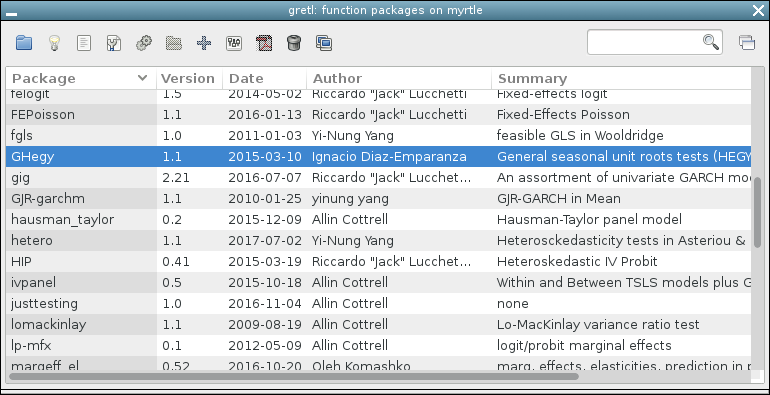
\includegraphics[scale=0.5]{figures/local-packages.png}
\end{center}
\caption{Browser for installed packages. It's quite easy to tell this
  apart from the ``on server'' window. Apart from their title-bars,
  this one has a lot more toolbar buttons (you can do more with a
  package once it is installed).}
\label{fig:local-packages}
\end{figure}

Returning to the installation process, to make sure what you've found
is really what you want, you can get more information on the package,
either by clicking on the ``Info'' icon (top-left in
Figure~\ref{fig:ghegy-lst}), or by right-clicking on the package entry
and selecting \textsf{Info} from the context menu. You'll be presented
with a window like Figure~\ref{fig:ghegy-info}.

\begin{figure}[htbp]
\begin{center}
  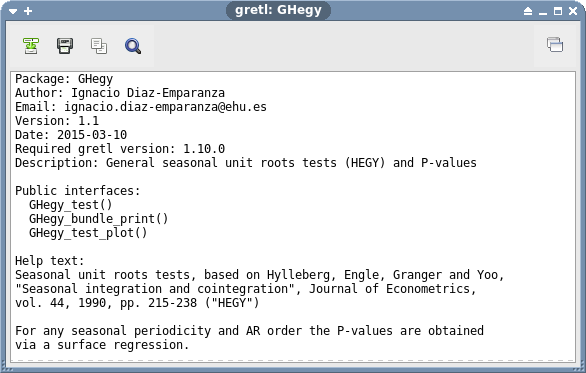
\includegraphics[width=0.65\textwidth]{figures/ghegy-info.png}
\end{center}
\caption{Get more info on GHegy}
\label{fig:ghegy-info}
\end{figure}

Yes, this definitely looks like it. At this point, all you have to do
is install the package: click on the ``Install'' icon in the browser
window, or, again, right-click on the package entry. Gretl will now
download the package from the sourceforge server and install it.

\begin{figure}[htbp]
\begin{center}
  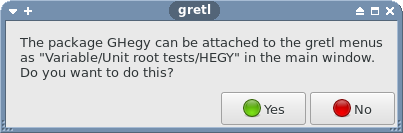
\includegraphics[width=0.4\textwidth]{figures/ghegy-menu.png}
\end{center}
\caption{Let GHegy attach to a menu?}
\label{fig:ghegy-menu}
\end{figure}

The final step of your installation is shown in
Figure~\ref{fig:ghegy-menu}.  Function packages may offer the option
of attaching to gretl's GUI menus: in this case, the author chose to
make it available among the other unit-root tests that gretl provides
natively. You may choose to accept this option (which makes it handy
to use the package from gretl's graphical interface) or not, if you
don't want to clutter up your menus with anything more than the
essential entries. Even if you say ``No'' here, however, the package
will still be available to you from the GUI interface---it just won't
have a dedicated menu entry. But note, this is not just a one-time
option; see Section~\ref{manage-menus} for an account of how to add or
remove installed packages from gretl's menus.\label{pg:menu-hook}

Suppose you say ``Yes'' to \textsf{GHegy}'s offer of a menu
attachment. Then the HEGY unit-root test should be available where
you'd expect to find it (Figure~\ref{fig:ghegy-hook}).\footnote{You
  used to have to restart the program to get such dynamic menu items
  to appear, but from gretl 1.10.2 that's no longer necessary.}

\begin{figure}[htbp]
\begin{center}
  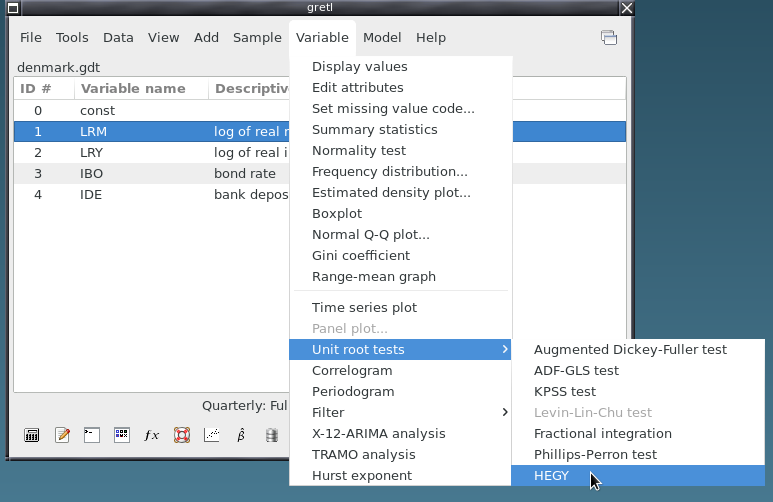
\includegraphics[width=0.8\textwidth]{figures/ghegy-hook.png}
\end{center}
\caption{The added menu item}
\label{fig:ghegy-hook}
\end{figure}

\subsection{Installing a package via the command line}
\label{sec:cli-install}

An alternative mechanism is provided by gretl's \cmd{pkg} command,
which can be invoked in the gretl console or in the command-line
program \app{gretlcli}. In its ``install'' mode this command has three
variants:

\begin{enumerate}
\item If you just type, for example,
%
\begin{code}
pkg install GHegy
\end{code}
%
  the presumption is that you mean to install a package named
  \textsf{GHegy} (either \texttt{.gfn} or \texttt{.zip}, that will be
  determined automatically) from the gretl server. So that's another
  way of doing what we just walked through, if you know in advance
  exactly what you want.
\item Suppose a colleague has given you a link to a function package
  that's not on the gretl server. Then you can download and install it
  on your own machine using the full URL, as in
%
\begin{code}
pkg install http://somewhere.net/gretl/splendid.gfn
\end{code}
%
\item Finally, suppose you have somehow got a copy of a function
  package independently of gretl: it's on your computer but not
  installed.  Then, to install it you want the \option{local} option
  (and you need to know the path to the file). So you might type
%
\begin{code}
pkg install /Users/Me/Downloads/splendid.gfn --local
\end{code}
%
\end{enumerate}

We have illustrated variants 2 and 3 of the \cmd{pkg} command
with \textsf{gfn} files, but note that they will also work for
packages in \textsf{zip} format.

\subsection{Updating a package}

Updating packages is easily done via the GUI. Look back at
Figure~\ref{fig:ghegy-lst}: in the rightmost column of the browser for
packages on the server you'll see a note of the local status of each
available package, either ``Up to date,'' ``Not installed'' or ``Not
up to date.'' (It may be necessary to expand the browser window or
scroll to the right in order to see this column.) It's a good idea to
visit this listing from time to time; if an installed package is
marked as not up to date, just click the Install button to update it.

\subsection{Uninstalling a package}

This is also easily and intuitively done via the GUI. From the
browser for locally-installed packages, select the package you want to
get rid of and click on the ``Unload/delete'' icon, or right-click to
the same effect.

You will be asked if you want to (a) unload the package from memory
(only) or (b) remove it from your system. The former might be useful
during an interactive session in which you want to clear up all the
functions you have in memory and start from scratch with no possible
confusion between functions you have written and those provided by a
package. The latter is of course more radical, and requires you to
reinstall the package if you change your mind.

Packages can also be removed via the command line: use the \cmd{pkg}
command with the name of an installed package plus \option{unload} or
\option{remove}. The former option unloads a package from memory and
also removes its menu attachment, if any (see
Section~\ref{manage-menus}); the latter option performs these actions
but also deletes the package file(s).


\section{Using function packages: the basics}

The browser window for installed packages has quite a rich set of
toolbar buttons and right-click context menu choices. If you're not
sure what a button might do, try mousing over it to get a ``tooltip.''
If you're still not sure, you might just try clicking it---gretl won't
do anything destructive without asking for confirmation first!

We'll discuss some of the less obvious choices in the window later,
but we would encourage you to explore.

\subsection{Using packages via scripting}

If you're interested in calling a function package via script you'll
probably want to examine its ``sample script.'' Hopefully this should
provide a useful template. Opening the sample script is one of the
options on right-clicking an installed package in the local package
browser.  Of course you should also read the help text for the
function you want to call.

You'll want to start your script by using the \cmd{include} command
to load the package in question, as in
%
\begin{code}
include GHegy.gfn
\end{code}

Note that even if a package comes in zip format, it's the \texttt{gfn}
file (which will be unpacked on installation) that you need to
include. It will always have the same basename as the zip package that
contained it.

The only effect of the \cmd{include} command above is to make the
functions contained in the package available to you. To use them, you
call them as if they were native gretl functions. So, for example, the
sample script for \textsf{GHegy} contains the following commands:

\begin{code}
include GHegy.gfn
open data9-3.gdt

# Tests with constant + dums + trend and fixed AR order 4,
# without printing the regression
bundle H1 = GHegy_test(reskwh, 0, 4, 3, 0)

# Tests with constant + dums, AR order determined by BIC with
# a maximum of 10, printing the regression
bundle H2 = GHegy_test(reskwh, 2, 10, 2, 1)
\end{code}

The purpose of the first two commands is obvious and needs no
comment. However, the two invocations of the \dtk{GHegy_test}
function may not be totally transparent. In general you should expect
some documentation on (a) which functions are contained in the package
and (b) their syntax: the parameters they accept, what they do, what
they return.\footnote{This is the responsibility of package authors.
  However, the gretl development team tries try to ensure that
  packages obtained via the gretl server contain at least minimal
  documentation.}  To find this, go to the list of locally-installed
packages and click on the ``Info'' icon. A text box will appear
showing the documentation provided by the package author. In the
\textsf{GHegy} case, for example, not only are we told all we need to
know about the \dtk{GHegy_test} function, but we also discover that
the package contains two additional functions that we can use, namely
\dtk{GHegy_bundle_print} and \dtk{GHegy_test_plot}.  So, for
example, we could use the latter to enhance Ignacio's sample script,
appending the line
%
\begin{code}
GHegy_test_plot(&H2)
\end{code}
%
Running it will then produce a graphic similar to the one displayed in
Figure~\ref{fig:ghegy-plot}.

\begin{figure}[htbp]
  \centering
  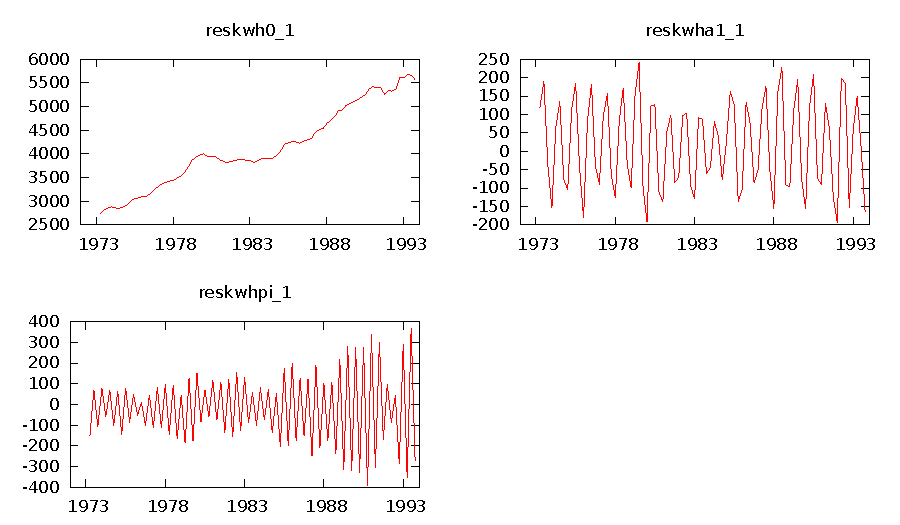
\includegraphics[scale=0.9]{figures/ghegy-plot}
  \caption{Output of the \dtk{GHegy_test_plot} function}
  \label{fig:ghegy-plot}
\end{figure}

Some more complex packages offer help documentation in PDF format, for
example the \textsf{DPB} package \citep[see][]{DPBwp}.  If such
documentation is available for a given package, the PDF button on the
local package browser toolbar becomes active when the package is
selected; clicking it will display the file in your default PDF
reader.

Other than that, there's not much to say here. For help on scripting
in general, see the \textit{Hansl Primer} \citep{hansl-primer}.

\subsection{Using packages via the GUI}
\label{sec:gui-using}

Of course, if a package offers to attach to a gretl menu, and you
accepted that offer when you installed the package (see
page~\pageref{pg:menu-hook}) then you should know where to find it.
But if a package doesn't have its own place in the menus, the
package browser is the place to go to invoke it by GUI means.

You can launch a package by double-clicking on it. What exactly
happens here depends on whether the package's data requirement is
met. Most packages require that a dataset is open, and some have more
specific requirements (time series data, or panel data).

If you have a suitable dataset in place you will get a dialog box to
specify arguments to the function, much as you would with a built-in
gretl procedure. (However, if the package offers more than one public
interface you may get an initial dialog asking you to choose a
particular function to call.) If the package's data requirement is not
met, you'll be told what's wrong and asked if you'd like to run the
sample script. This should load suitable data and ``demo'' the
package.\footnote{If a package's sample script does \textit{not} run
  correctly, please report that to the author of the package or the
  \texttt{gretl-users} mailing list. Although gretl function packages
  carry no warranty it is supposed to be a firm requirement that the
  sample script runs OK.}

\begin{figure}[htbp]
  \centering
  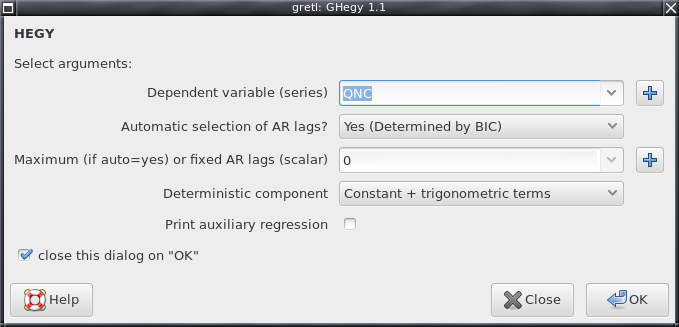
\includegraphics[width=0.7\textwidth]{figures/ghegy-call}
  \caption{GUI call to the \textsf{GHegy} package}
  \label{fig:ghegy-call}
\end{figure}

Figure~\ref{fig:ghegy-call} illustrates a function-call dialog, this
one put up by the \textsf{GHegy} package. Each argument to the
function is represented by either a drop-down selector or a check
box. Note that the ``\textsf{+}'' button next to a selector allows you
to define a new variable as an argument if you
wish. Figure~\ref{fig:ghegy-output} then shows part of the output from
this call.

\begin{figure}[htbp]
  \centering
  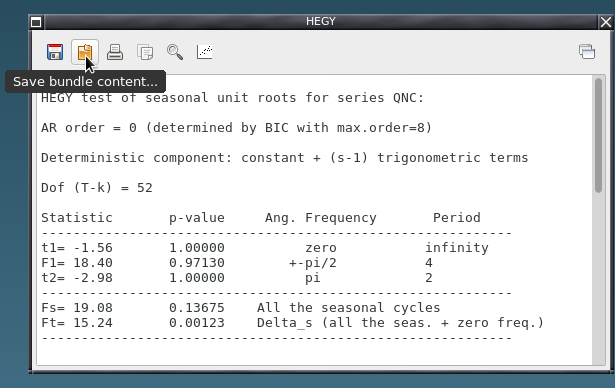
\includegraphics[width=0.7\textwidth]{figures/ghegy-output}
  \caption{Output window from call to \textsf{GHegy}}
  \label{fig:ghegy-output}
\end{figure}

We have moved the mouse pointer over the ``bundle'' icon in the
toolbar of this window to reveal the tooltip, ``Save bundle content.''
What's going on here is that \textsf{GHegy} has constructed a gretl
bundle containing various details of the unit root test, and you can
extract these details if you wish. Package authors: for an account of
how to enable this sort of thing see Section~\ref{sec:idioms}.


\section{Some finer points}
\label{sec:finer}

\subsection{Managing menu attachments}
\label{manage-menus}

We mentioned above that you can revise your initial choice of whether
or not to have a function package insert itself into the gretl
menus. We'll now explain how.

Again, start from the browser for installed packages. One of the
buttons on the toolbar is a ``\textsf{+}'' icon (with tooltip ``Add to
menu''). This button should be active when you select a package which
offers a menu attachment but is not currently attached. Click it and
you'll get the sort of dialog shown above in
Figure~\ref{fig:ghegy-menu}; say ``Yes'' to attach the package to the
specified menu.

To go the other way---that is, remove a package from a menu---use the
button with the ``Preferences'' icon (tooltip ``Package
registry''). This brings up a window showing the packages that are
currently attached to menus (Figure~\ref{fig:pkg-registry}). For each
package you can see whether its attachment is in the main gretl window
or in model windows (at present these are the only two possibilities),
as well as the specific ``path'' to the menu item. To remove a package
from the menus, use the delete button or the right-click
menu. Removing a package from the menu system does not delete or
disable the package, it just means it won't have its own menu
item---which is easily reversed, as we have just seen.

\begin{figure}[htbp]
  \centering
  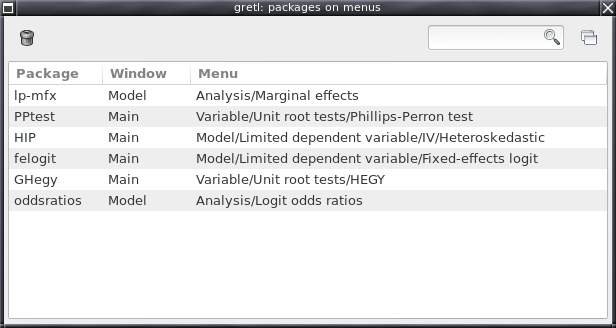
\includegraphics[width=0.7\textwidth]{figures/pkg-registry}
  \caption{The GUI package ``registry'': from here you can remove
    dynamic menu items}
  \label{fig:pkg-registry}
\end{figure}

Changes made in this way will have immediate effect on main-window
menus; the effect on model-window menus will be apparent only for
newly opened windows.

\subsection{What does ``installed'' mean?}
\label{sec:installed}

We've talked about installing packages, but what exactly does it mean
for a package to be installed? Basically, it means that the package
file(s) are placed in one or other of two standard locations where
gretl should always be able to find them automatically---for example,
in response to the command ``\texttt{include mypkg.gfn}'' without any
path specification.

These two standard locations are the ``system'' and ``per-user'' gretl
function directories. In each case we're talking about a subdirectory
named \texttt{functions}, the actual path to which differs by platform
(and on MS Windows, by national language).

On an English-language Windows installation typical values are, for
the system and per-user paths respectively,
%
\begin{code}
C:\Program Files\gretl\functions
C:\Users\login\AppData\Roaming\gretl\functions
\end{code}
%
where ``login'' is a placeholder for your username. On Linux they are
likely to be
%
\begin{code}
/usr/share/gretl/functions
$HOME/.gretl/functions
\end{code}
%
and on Mac OS X
\begin{code}
/Applications/Gretl.app/Contents/Resources/share/gretl/functions
$HOME/Library/Application Support/gretl/functions
\end{code}
%
where
\verb|$HOME| is your ``home'' directory, which is always defined on
Linux and OS X.

However, you don't need to guess at these locations: in the gretl
console you can do
%
\begin{code}
eval $gretldir
eval $dotdir
\end{code}
%
to get the respective base directories on your system: append
``\texttt{functions}'' and you'll have the canonical package
paths.\footnote{OK, there's an exception here: on Mac OS X the path to
  the per-user functions directory, which is shown above, is not the
  same as the \verb|$dotdir| path.}

When you install a package via gretl it will go to one of these
locations, depending on the platform and whether or not you have
permission to write to the ``system'' directory.

We said gretl will automatically find packages in these places. Well,
there's one possible catch to look out for. The \texttt{gfn} file for
a package may be placed in the \texttt{functions} directory itself, or
in a subdirectory with the same name as the package; that is, on one
or other of the following patterns:
%
\begin{code}
functions/mypkg.gfn
functions/mypkg/mypkg.gfn
\end{code}
%
Why the difference? If a package includes PDF documentation, or any
other files besides the \texttt{gfn}, \textit{it must be in its own
  subdirectory} (the second pattern). But if the package consists of a
gfn file only, then it should go directly into the \texttt{functions}
directory (the first pattern).  Gretl should get this right when
installing a package for you but if you install a package by hand,
copying it to the \texttt{functions} directory yourself, you should
pay attention to this point.

\subsection{Examining a package in depth}

Suppose you get seriously interested in some function package: you
don't just want to use it, you want to see how it works, maybe borrow
ideas from it, even fix bugs in the package or modify it for your own
purposes.\footnote{If you do come up with any fixes or enhancements,
  then naturally we ask that you share them with the package author.}

Once again, you can start from the browser window for packages ``on
local machine.'' The \textsf{View code} button or right-click menu
item brings up a window showing all the function code. From here
you may copy material and paste it into a script of your own.

Making changes to an existing package, however, cannot be done via the
package browser window: it's necessary to go via the main-window menu
item ``File, Function packages, Edit package.'' This route will let
you edit a package only if you have write permission on the file in
question.  Here's a plausible scenario: you have package \textsf{XYZ}
installed, and you don't want to (or don't have permission to) mess
with the installed version, but at the same time you'd like to do some
exploration and/or experimentation. Solution: go to the web interface
to gretl packages mentioned in Section~\ref{sec:browsers} and download
a copy of \textsf{XYZ}, placing it somewhere other than one of the
standard gretl function directories. Then go to ``File, Function
packages, Edit package...'' and navigate to find the \texttt{gfn}
file. (If the package is in zip format you'll have to unzip it first.)

In the package editor window, the button labeled \textsf{Edit function
  code} takes you into the hansl code (function by function, if the
package contains more than one function). With a complex,
multi-function package it may be difficult to get a good overview of
the package in this way but here's an alternative: click the
\textsf{Save...} button and select \textsf{Save as script}. This
enables you to write out a gretl \texttt{inp} file containing all the
functions in the package, which you can then open in gretl's script
editor---or, of course, the text editor of your choice.

An alternative way of opening a specific package for editing, via the
command line in a terminal window, is to invoke gretl with the flag
\texttt{-p} plus the name of the package, as in
%
\begin{code}
cd XYZ_work_dir
gretl -p XYZ.gfn
\end{code}
%
Either way, opening the specified \texttt{gfn} file for editing has
the effect of loading the package into memory. Thereafter, operations
related to \textsf{XYZ} will refer to the version you loaded
initially.

\subsection{Redirecting the package browser}

Another way of getting at uninstalled \textsf{gfn} files is to
redirect the function package browser. This can be done via the
directory button at the left-hand end of the toolbar, which calls up a
selection dialog. If you select a directory that turns out to contain
no \textsf{gfn} files you just get a message to that effect, otherwise
you are given the option of replacing the original contents of the
browser window with the newly found packages.

When the browser is redirected in this way, clicking the directory
button gives you two options: choose another directory, or revert to
displaying the installed packages (which may come from more than one
directory, as explained in Section~\ref{sec:installed}).

When the browser is newly opened it always shows the installed
packages. However, gretl will remember (during a given session) which
alternative \textsf{gfn} directory you visited last, and will offer
that as the default selection on using the directory button.

%% \subsection{Debugging a package}
%%
%% To be written---but maybe move to the ``authoring'' chapter?

%%%%%%%%%%%%%%%% chapter break %%%%%%%%%%%%%%%%%

\chapter{For package authors}
\label{chap:authors}

Recall from Section~\ref{sec:pkgform} that the core elements
of a gretl function package are as follows:
\begin{enumerate}
\item One or more hansl functions;
\item the package metadata (author, version and so on);
\item documentation; and
\item an example script.
\end{enumerate}
These elements are all contained in a \texttt{gfn} XML file.
Optionally, you can ship additional material with your package (PDF
documentation, a richer assortment of sample scripts, and so forth),
in which case all the components including the \textsf{gfn} must be
wrapped in a zip file.

In this chapter, we will go through the creation and maintenance of
these basic ingredients, plus the process of baking them together into
a working function package. This result can be achieved either by
command-line methods or via gretl's graphical interface.

We'll start with the command line. Yes, we know that many readers may
prefer to use a graphical interface whenever possible, but we
recommend that you at least skim this section rather than skipping
forward.  The command-line approach is likely to pay off if you ever
decide to tackle an ambitious function-package project.

% (\ref{sec:gui-build}). Section~\ref{sec:common-req} covers some common
% requirements that are important regardless of how the package is
% built.

\section{Building a package via the command line}
\label{sec:cli-build}

Here we assume you are at least somewhat familiar with the
``shell''---that is, the command processor which awaits your input
when you open a terminal window. So we assume you know how to perform
simple operating-system tasks such as copying/deleting files, listing
the contents of a directory and so on via the appropriate shell
commands. A reminder of the basics is provided in
Table~\ref{tab:basics}. On unix-type systems (such as Linux and OS X)
you can get help on a command by typing man followed by the command
word, as in \texttt{man cp}. On windows, get help by typing the
command word followed by a slash and a question mark, as in
\texttt{copy /?}.

\begin{table}[htbp]
\centering
\begin{tabular}{lll}
\textit{action} & \textit{unix} & \textit{Windows} \\[4pt]
copy file(s) & \texttt{cp} & \texttt{copy} \\
move files(s) & \texttt{mv} & \texttt{move} \\
delete files(s) & \texttt{rm} & \texttt{del} \\
make a directory & \texttt{mkdir} & \texttt{mkdir} \\
change directory & \texttt{cd} & \texttt{cd} \\
list files & \texttt{ls} & \texttt{dir} \\
emit a string & \texttt{echo} & \texttt{echo}
\end{tabular}
\caption{Basic shell commands by platform}
\label{tab:basics}
\end{table}

With the exception of subection~\ref{sec:using-make} all the commands
used in this section have been tested on Windows' \app{cmd.exe} as
well as the \app{bash} shell.

First of all, we strongly recommend that when starting work on a
package you create a specific directory to hold the makings of the
package. For illustration we'll suppose the package is called
``mypkg''. (You should, of course, replace all occurrences of
\texttt{mypkg} below with the actual name of the package you're
building.) So, starting from some suitable point in your file system,
you might begin with
%
\begin{code}
mkdir mypkg
cd mypkg
\end{code}

Now, the minimum requirement for building your package (as a ``simple
package'' or stand-alone \textsf{gfn} file) is the following set of
files:
\begin{enumerate}
\item At least one (for now, let's say one) hansl \textsf{inp} file
  containing definitions of the functions you wish to package. Let's
  call this \texttt{mypkg.inp}.
\item A \textsf{spec} file, which supplies metadata and tells gretl how the
  package should be assembled; call this \texttt{mypkg.spec}.
\item A sample script (\textsf{inp} file) which exercises your
  package; call this \dtkttt{mypkg_sample.inp}.
\item A text file containing help on the packaged function(s). Call
  this \dtkttt{mypkg_help.txt}, or preferably \dtkttt{mypkg_help.md}
  if you're going to use gretl's markdown option (which is
  recommended: see Section~\ref{sec:md} below).
\end{enumerate}

The four files listed above are all UTF-8 text files that you can view
and modify using any text editor of your choice (no word processors,
please). Each text file corresponds to one of the four basic
constituents of a \texttt{gfn} file. Therefore, once you have these
four files ready, building the package is simply a matter of
transcribing their contents into XML and putting everything together
into the package file.

You will need to create such files in the current directory (or maybe
copy or move them from elsewhere if you've already made a start). It's
not absolutely necessary that \textit{all} the filenames are
regimented as shown (starting with the name of the package in each
case), but as we'll see shortly this can make life easier.

The \textsf{inp} file containing your function definitions we won't
say much about here. If you're contemplating writing a package you
should already be pretty comfortable with hansl. See the \textit{Hansl
  Primer} \citep{hansl-primer} if in doubt.

The requirements on the sample script and help text are set out in
Section~\ref{sec:common-req}.  First we'll deal with the \textsf{spec}
file. A simple case of this is shown in Listing~\ref{ex:spec1}.

\begin{script}[htbp]
  \caption{Simple \texttt{mypkg.spec}}
  \label{ex:spec1}
\begin{code}
author = A. U. Thor
email = author@somewhere.net
version = 1.0
date = 2018-07-12
description = Suitable description goes here
tags = C13
public = myfunc
help = mypkg_help.md
sample-script = mypkg_sample.inp
min-version = 2017a
\end{code}
\end{script}

According to this spec, the package has a single public function,
\texttt{myfunc}, and requires gretl 2017a or higher to run
correctly. Writing a \textsf{spec} from scratch may be tricky. Please
refer to chapter~\ref{chap:specfile} for a fuller account of the
various keywords, and in particular Section~\ref{sec:spec-basic} for
the obligatory basics.

Now, assuming all the required files are in place, how do we actually
build the package? Simple: the shell command
%
\begin{code}
gretlcli --makepkg mypkg.inp
\end{code}
%
tells \textsf{gretlcli} to run \texttt{mypkg.inp}, hence loading your
function definitions into memory; process the corresponding
\textsf{spec} file (which must have the same basename as the
\textsf{inp} file); load the auxiliary files (help, sample script);
and, if all goes well, write out \texttt{mypkg.gfn}. For reference,
using the \option{makepkg} flag with \app{gretlcli} is just a
convenient shorthand: it's equivalent to running the following script,
using the \cmd{makepkg} command.
%
\begin{code}
include mypkg.inp
makepkg mypkg.gfn
\end{code}
You can further abbreviate the above by using the ``short'' syntax for
options, as in
\begin{code}
gretlcli -m mypkg.inp
\end{code}

We've said this package offers a single public function,
\texttt{myfunc}: that's the only function that will be made directly
available to users. However, you may want to include one or more
private ``helper'' functions, designed to be called only by
\texttt{myfunc}. To do so, just put definitions of these functions
into \texttt{mypkg.inp}; \textsf{gretlcli} will pick them up and,
seeing that they don't appear in the \texttt{public} listing, will
mark them as private.\footnote{To be quite explicit, the
  \texttt{makepkg} mechanism includes in the output package all the
  functions that are currently in memory---as package-private
  functions if they are not identified as public in the \textsf{spec}
  file. When using \texttt{makepkg} you should always start with a
  clean workspace and load only the relevant functions.}

\subsection{The markdown option}
\label{sec:md}

As mentioned above, a simple function package includes documentation
in the form of a text file. Since gretl 2023b you can employ a simple
variant of markdown, and we encourage package authors to do so. If you
are unfamiliar with markdown you might want to take a look at
\url{https://en.wikipedia.org/wiki/Markdown}.

Gretl's markdown variant currently supports the following features.

\begin{itemize}
\item First and second-level headings: start a (single) line with
  \verb|#| or \verb|##|, respectively
\item Boldface: \verb|**text**|
\item Italic: \verb|*text*| or \verb|_text_|
\item Monospace: \verb|`text`| (enclosed in ASCII left quotes)
\item Itemized list: each item starts with ``\verb|- |'' on a new line
\item Enumerated list: each item starts with (e.g.) ``\verb|1. |''
  on a new line
\item Code block: starts and ends with \verb|```| (three ASCII left
  quotes) on its own line
\end{itemize}

Note that itemized and enumerated lists cannot be nested, and a blank
line should be inserted before starting an itemized list, an
enumerated list, or a code block.

URLs starting with \texttt{http[s]} automatically turn into
hyperlinks.  Paired ASCII straight double quotes are automatically
replaced by left- and right-hand quotes.

\subsection{Adding extra material}

Suppose now that you want to include with your package some extra
material (say, a specialized data file). As explained earlier (again,
see Section~\ref{sec:pkgform}), you will have to create a suitably
organized zip file.

The first thing is to update the \texttt{spec} file to refer to the
extra content: you'll want to add a line like
\begin{code}
data-files = somedata.gdt
\end{code}
where we assume that the file \texttt{somedata.gdt} file exists and is
in the \texttt{mypkg} directory. See Section~\ref{sec:spec-extra} for
more details.

Creating the zip file can be done ``by hand'' if the command-line
\textsf{zip} program is available (or substitute \textsf{pkzip} if
it's available):
\begin{code}
cd ..
zip mypkg/mypkg.zip mypkg/ mypkg/mypkg.gfn mypkg/somedata.gdt
\end{code}

Or you can have gretl take care of everything for you, by using the
\cmd{makepkg} command: you can start \app{gretlcli} and issue the
following command:
%
\begin{code}
makepkg mypkg.zip
\end{code}
%
When the argument to \cmd{makepkg} is a filename with the \textsf{zip}
extension, gretl will do one of two things:
\begin{itemize}
\item If a matching \textsf{gfn} file is found, this will be used the
  as the basis for the zipfile, with other components pulled in as
  specified.
\item Failing that, if a matching \textsf{spec} file is found (plus
  the other files that it references), gretl will first build the
  \textsf{gfn} and then build the zipfile wrapper.
\end{itemize}

A neater way of doing this is to ``pipe'' the \cmd{makepkg} command
into \app{gretlcli} directly from the command line, as in
\begin{code}
echo makepkg mypkg.zip | gretlcli -b -
\end{code}
%
where the \texttt{-b} flag makes \textsf{gretlcli} operate
non-interactively and the following dash tells the program to read
commands from ``stdin'' instead of an \textsf{inp} file.

\subsection{Using a Makefile}
\label{sec:using-make}

If you're working on a platform that supports the \app{make} utility,
you might find a Makefile helpful. It is not obligatory to use this
approach, but especially if your project is large, it can definitely
make your life easier. MS Windows does not provide \app{make}, but it
can be installed; see Appendix A to this chapter for some options.

\app{Make} is a program that gives you a consistent interface for
performing complex tasks. Its usefulness is particularly evident when
there is some dependency structure between the tasks you want to
perform. For example, when building a large software project, there is
a series of operations that must be performed in a certain order
(compiling, linking, installing); or, as another example, when you
have a large \LaTeX{} document you have to compile it first, then run
\BibTeX{}, then compile it again, etc. \app{Make} is excellent at
automating such tasks.

To run \app{make} you need a file, usually called \texttt{Makefile},
which contains a sequence of rules to tell the program ``what to do
when.''\footnote{A complete tutorial on \app{make} can be found at
  \url{http://www.gnu.org/software/make/manual/make.html}.}
Listing~\ref{ex:make1} shows a very simple instance, though it does
illustrate a small refinement in the package-building process.

\begin{script}[htbp]
  \caption{Makefile for simple package}
  \label{ex:make1}
\begin{code}
PKG = mypkg

$(PKG).gfn: $(PKG).inp $(PKG).spec $(PKG)_help.txt $(PKG)_sample.inp
	gretlcli --makepkg $(PKG).inp

install: $(PKG).gfn
	echo pkg install $(PKG).gfn --local | gretlcli -b -

clean:
	rm -f $(PKG).gfn
\end{code}
\end{script}

Running ``\texttt{make}'' in your project directory will rebuild
\texttt{mypkg.gfn} if and only any of the source files have changed
since the \textsf{gfn} was last produced; running ``\texttt{make
  clean}'' will delete the \textsf{gfn}. Here's the refinement:
running ``\texttt{make install}'' will install the package (after
rebuilding it, if required).

Warning: if you just copy and paste the example above into a text
file, chances are it will not work. \app{Make} is quite fussy about
the structure of the Makefile, particularly about the use of tabs
versus spaces. Some details, and a more extended example, are provided
in Appendix B to this chapter.

\section{Building a package via the GUI}
\label{sec:gui-build}

When you're building a package, it's a good idea to ensure you have a
``clean'' workspace. So if you've been running regressions, maybe
using other packages, or whatever, we recommend saving your work,
closing gretl, and restarting the program.  That said, here's a
walk-through of the process.

\subsection{Load at least one function into memory}

If you have a script file containing relevant function definitions,
open that file and run it. Otherwise you can create a script file from
scratch in the GUI script editor: include at least one function
definition, and run the script.

For example, suppose you decide to package a function that returns the
percentage change of a time series.\footnote{Strictly as an
  illustration, of course! Don't expect something like this to pass
  muster for inclusion on the gretl server.} Open the script editor
window and type
%
\begin{code}
function series pc(series y "Series to process")
    series ret = 100 * diff(y)/y(-1)
    string dsc = sprintf("Percentage change of %s", argname(y))
    setinfo ret --description="@dsc"
    return ret
end function
\end{code}

Note that we have appended a string to the function argument, so as to
make our interface more informative.  This is not obligatory: if you
omit the descriptive string, gretl will supply a predefined one (in
this case, \texttt{series}).

\begin{script}[htbp]
  \centering
  \begin{scode}
              x         dpcx

 1    0.4428625
 2    0.3737993     -15.5947
 3    0.1570864     -57.9757
 4    0.6896227     339.0086
 5    0.8510148      23.4030
 6      0.07757     -90.8851
 7    0.1454557      87.5180
 8    0.8260684     467.9174
 9    0.4328073     -47.6064
10    0.3566473     -17.5967

  \end{scode}
  \caption{Output of function check}
  \label{ex:func_check}
\end{script}

Now run your function. You may want to make sure it works properly by
running a few tests. For example, you may open the console and type

\begin{code}
series x = uniform()
series dpcx = pc(x)
print x dpcx --byobs
\end{code}

You should see something similar to Listing~\ref{ex:func_check}. The
function seems to work OK.  Once your function is debugged, you may
proceed to the next step.

\subsection{Create your package}
\label{sec:gui-create}

In the gretl main window, go to the ``File, Function packages'' menu,
and select ``New package.''  A first dialog should appear (see
Figure~\ref{fig:startpkg}), in which the left-hand panel lists all the
functions you have available for packaging; you must specify the name
of the package, one or more public functions to package, and zero or
more ``private'' helper functions.

\begin{figure}[htbp]
  \centering
  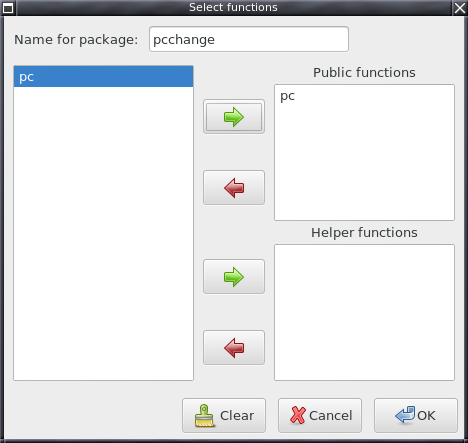
\includegraphics[scale=0.5]{figures/newpkg}
  \caption{Starting a new function package: you specify a name for the
    package and select the functions to be included from the list on
    the left.}
  \label{fig:startpkg}
\end{figure}

Public functions are directly available to users; private functions
are part of the ``behind the scenes'' mechanism in a function
package. So, at this point, you select the \cmd{pc} function from the
left-hand panel and put it into the ``Public functions'' box. You also
give the package a name. Leave off the \texttt{gfn} extension, that
will be added as required; here we name the package \texttt{pcchange}.

\begin{figure}[htbp]
  \centering
  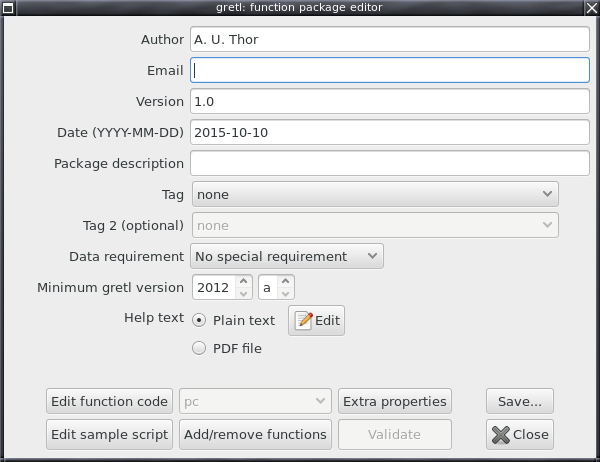
\includegraphics[scale=0.55]{figures/package_editor}
  \caption{The package editor window}
  \label{fig:package_editor}
\end{figure}

On clicking \textsf{OK} a second dialog should appear (see
Figure~\ref{fig:package_editor}), where you get to enter the package
information (author, email, version, date, etc.). Unless you have a
PDF file containing help, you should also enter help text for the
public interface: use the \textsf{Edit} button to open a text entry
window. (If you have documentation in PDF format, see
Section~\ref{sec:gui-pdf}.) You have a further chance to edit the code
of the function(s) to be packaged, by clicking on \textsf{Edit
  function code}.  (If the package contains more than one function, a
drop-down selector will be shown.)

And you get to (in fact, you \textit{must}) add a sample script that
exercises your package.  This will be helpful for potential users, and
also for testing. For this package, a suitable sample script might
looks like this:
%
\begin{code}
include pcchange.gfn
open denmark.gdt
series pcLRM = pc(LRM)
print LRM pcLRM --byobs
\end{code}
%
where (a) we've decided that the package is to be called
\textsf{pcchange}, and (b) we're going to illustrate using S\o{}ren
Johansen's Danish macroeconomic data (included with the gretl
package). See Section~\ref{sec:common-sample} for details on what's
required of a sample script.

At this point you should also consider the metadata items
\textsf{Minimum gretl version}, \textsf{Data requirement} and
\textsf{Tag}.  You can read all about these in
Section~\ref{sec:spec-basic}. For the moment, suffice it to say that
since the function code above doesn't do anything exotic you may be OK
leaving the minimum gretl version at its default value, though if you
want to check when some function or command was introduced you can
look at the gretl ChangeLog.\footnote{See
  \url{http://gretl.sourceforge.net/ChangeLog.html}.} As for the data
requirement, well, percentage changes from observation to observation
probably don't make sense for cross-sectional data (which in most
cases can be ordered any old how, arbitrarily), so you might pull down
the list of options and select ``Time-series data.'' And as regards
the tag for this package, the most general category, ``C10 Econometric
and Statistical Methods: General'' is probably the only one that's
applicable.

Clicking the \textsf{Save} button in the package editor window brings
up a little menu. At this stage it's just the first item, \textsf{Save
  gfn}, that's relevant. If there's something missing from your
package specification (e.g.\ no help text), you'll get a nag box when
you select this item. Otherwise you'll see a dialog where you get to
choose whether to save the \textsf{gfn} file to an ``installed''
location (see Section~\ref{sec:installed}) or in some other place
(Figure~\ref{fig:gfnsave}).

\begin{figure}[htbp]
  \centering
  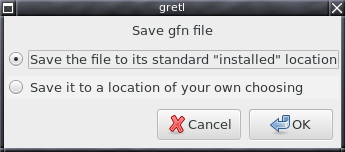
\includegraphics[scale=0.45]{figures/gfnsave}
  \caption{Where do you want your new package to go?}
  \label{fig:gfnsave}
\end{figure}

If you select the first option you will get feedback on where the gfn
file was actually written;\footnote{Technical note: this option will
  take care of saving the \textsf{gfn} to a named subdirectory of the
  relevant \texttt{functions} directory, if the specification includes
  PDF documentation or other additional files.} if you select the
second you'll get a regular File Save dialog box. The advantage of the
first choice is that the package will be found automatically by gretl.
However, if you're just experimenting and don't want to ``install''
the package yet, by all means choose a different location.

Note that the dialog box shown in Figure~\ref{fig:gfnsave} only
appears when you are first saving a newly created package. Thereafter,
\textsf{Save gfn} simply saves the package using the existing path to
the \textsf{gfn} file.

\subsection{Adding PDF documentation}
\label{sec:gui-pdf}

The prerequisite here is that you have available a suitable PDF file
containing documentation for your package. We can't help you with
that. But if you have such a file, then click on the \textsf{PDF file}
radio button to the right of the ``Help text'' field in the package
editor. If you have already entered plain-text help you will see a
dialog box warning you that this will be lost (not right away, but if
and when you save the package). Otherwise you go straight to a file
chooser window where you select the PDF file.

To be included with your package, the PDF file must (a) be in the same
location as the \textsf{gfn} file, and (b) have the same ``basename''
(for example \texttt{mypkg.pdf} if the package is called
\textsf{mypkg}). Nonetheless, you can select a PDF file of any name
from any location, and gretl will take care of copying it into place
under the correct name. But please note: if gretl has to copy the file
into place, any changes made to the PDF in its original location will
\textit{not} propagate to the copy included in the package. Having
selected PDF documentation, however, you can use the \textsf{Select}
button (see Figure~\ref{fig:package_editor}) to check where gretl is
finding the file, or to update it from another location.

Please note: PDF help is an \textit{alternative} to plain text
help; you cannot combine the two (not at present, anyway).

\subsection{Saving a zip file}
\label{sec:save-zip}

In the little menu that is brought up by the \textsf{Save} button in
the package editor window, one of the items is ``Save zip file...''.
This item becomes active if and only if the following conditions are
satisfied:
\begin{itemize}
\item Your package offers PDF documentation and/or additional data
  files. That is, the specified materials can't all be packed into the
  straight \textsf{gfn} XML format.
\item The \textsf{gfn} file is up-to-date with any current changes
  made in the package editor.
\end{itemize}
If you think you ought to be able to save a zip file but that option
is not enabled, chances are the \textsf{gfn} file needs to be saved
first (to keep things in sync).

\subsection{Check your package!}

Before sharing your package with others, you must check that it
actually works, outside of the package-editing context. You need to
emulate the context of somebody who has installed your package from
scratch.

First off, that means that if you didn't choose to write your package
into a standard location at the step in Section~\ref{sec:gui-create}
you should do so now. Use the ``Save...'' button in the GUI package
editor or see Section~\ref{sec:cli-install} for other options.

Once your package is in the right place, close gretl then reopen it.
Now go to ``File, Function packages, On local machine''. If all has
gone OK so far, you should see the file you packaged and saved, with
its short description.  If you click on ``Info'' you get a window with
all the information gretl has gleaned from the package.  If you click
on the ``View code'' icon in the toolbar of this new window, you get a
script view window showing the actual function code. Fine.

Now, back to the ``Function packages'' window. Think for a moment: you
required time-series data (didn't you?) so you should know that a
double-click on your package will just offer the option of running
your sample script if time-series data are not loaded
(Section~\ref{sec:gui-using}). And if you're following directions you
have no dataset open at present. OK, it's worth trying that; your
sample script really, really should work regardless
(Section~\ref{sec:common-sample}), so go ahead and
double-click.\footnote{By the way, here's another thing: after loading
  the function(s) from the package, open the GUI console. Try typing
  \texttt{help pc}: the help text you entered should be presented.}

Now, if that went OK, let's next try a ``clean'' invocation of your
function. (Close and restart gretl if you've messed with your package
at all in the interim.)  First we'll load suitable data---preferably
something different from the sample script, for example the file
\texttt{np.gdt} (From Nelson and Plosser, also supplied with gretl
among the sample datasets, under the \textsf{Gretl} tab). We'll
compute the rate of change for the variable \texttt{iprod} via your
new function and store the result in a series named \texttt{foo}.

Return to ``File, Function packages, On local machine,'' find your
package, and double-click on it. A window similar to that shown in
Figure~\ref{fig:function_call} will appear.  Notice that the
description string ``Series to process,'' supplied with the function
definition, appears to the left of the top series chooser.

\begin{figure}[htbp]
  \centering
  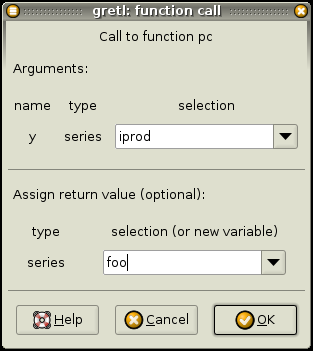
\includegraphics[scale=0.5]{figures/function_call}
  \caption{Using your package}
  \label{fig:function_call}
\end{figure}

Click \textsf{OK} and the series \texttt{foo} will be generated. Yay!
See Figure~\ref{fig:iprod_pc} (right-click on \texttt{foo} in the
gretl main window and choose \textsf{Time series plot}).

\begin{figure}[htbp]
  \centering
  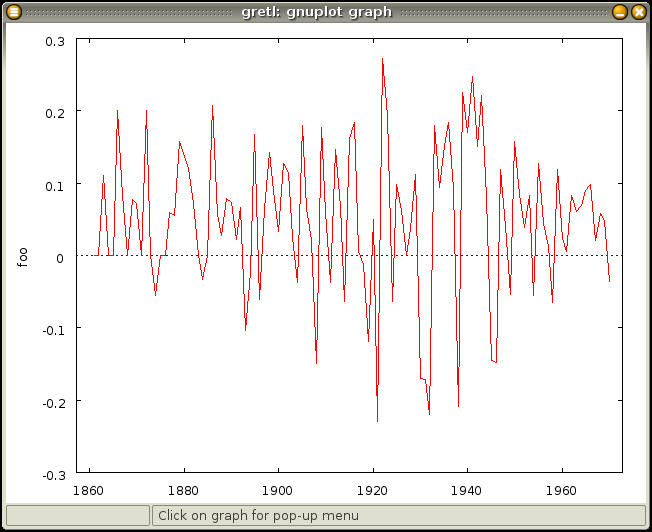
\includegraphics[scale=0.6]{figures/iprod_pc}
  \caption{Percent change in industrial production}
  \label{fig:iprod_pc}
\end{figure}

\section{Common requirements}
\label{sec:common-req}

Whether you're building a function package from the command line or
composing a package via the gretl GUI, certain requirements must be
met if your package is to be made available via the gretl server. Here
we spell out what's needed in regard to the help text and the sample
script.

\subsection{Help text}

This must give a clear (if brief) account, in English, of what the
package does, and also what each parameter does, for each public
function, insofar as explanation is reasonably required. (A boolean
\texttt{verbose} parameter probably doesn't need much if any comment,
but most parameters do need comment.)

If the help is not in PDF format it must be encoded in UTF-8 (or plain
ASCII, which is a proper subset of UTF-8). Unless you use the markdown
option (see Section~\ref{sec:md}) we recommend that lines of plain
text are kept to around 70 characters in width: some people may like
to run gretl windows at full-screen size, but many of us do not!

\subsection{Sample script}
\label{sec:common-sample}

This is crucial. The sample script \textit{must} work ``out of the
box'' on all platforms, and \textit{must not} take too long to
execute.

The sample script is what curious users are likely to run if they just
want to see what a package does and check that it's not broken. It's
what we gretl developers want to run for the same reasons, but also in
the process of regression-testing new gretl release candidates. It's
important that a gretl release doesn't break existing packages,
but we can't assess that if a package's sample script is broken in the
first place.

Here are the key things to watch out for in relation to sample
scripts:

\vspace{1ex}
\textit{Include yourself}: Right at the top, the sample script
  must \texttt{include} the \texttt{gfn} file in question. This will
  never do any harm, and is needed when the script is run ``from
  scratch'', without the package being already loaded.  The name of
  the \texttt{gfn} file should be given without any added path, and
  without quotation marks, as in

  \texttt{include mypkg.gfn}

\vspace{1ex}
\textit{Dataset}: If the package requires that a dataset be in
  place the sample script \textit{must} arrange for this in a portable
  manner. The options are as follows.
 \begin{enumerate}
 \item Open a data file that's supplied with the gretl distribution
   (that is, under the \textsf{Gretl}, \textsf{Greene} or
   \textsf{Ramanathan} tabs in the built-in datafile browser).
   But if none of the supplied data files are suitable, then
 \item construct an artificial dataset using the \texttt{nulldata}
   command and gretl's random-number generation facilities, or
 \item specify a downloaded data file using the \texttt{http} prefix
   with the \texttt{open} command, or
 \item include a suitable data file in your package---this requires
   that the package be in zip format.
 \end{enumerate}
 In the case of artificial data, the script should include a
 \texttt{set seed} command so that the results are reproducible. In
 the case of downloaded data the URL should be reasonably stable, not
 something that's likely to disappear or be moved before long.

 In no case should a datafile be specified with a full path, as in
 \begin{code}
 open /usr/share/gretl/...       # No!
 open C:\Program Files\gretl\... # No!
 \end{code}
  This is obviously not portable, and is never necessary when opening
  a supplied data file, given gretl's path-searching capability.

\vspace{1ex}
\textit{Execution time}: Some packages carry out Monte Carlo
  analyses and/or bootstrapping and we all know that such procedures
  are inherently time consuming. Nonetheless, a sample script should
  execute on current hardware in a reasonably short time---preferably
  less than 15 seconds and certainly less than a minute. Otherwise
  both casual users and testers will lose patience. If this means that
  only a ``toy'' example can be run, that's OK. The author can add
  comments to the script saying that this is just an illustration,
  serious use requires many more iterations. And/or one can add a more
  ``realistic'' invocation of the function(s), commented out, with a
  statement such as ``Uncomment this for a real test''.

\vspace{1ex}
\textit{Commenting out}: In some cases an author may wish to
  indicate alternative ways of calling his or her package. That's
  fine, but if an alternative call requires a dataset other than
  the one opened by the script it must be commented out; we don't
  want any lines in the sample script that will generate errors
  when the script is called ``as is''.

\vspace{1ex}
The intent of the sample script in a gfn package is not just ``a rough
idea of how you might call this package'', or ``something that ran OK
for the author on some machine at some time'', but something that will
run for any user of gretl on any platform, without modification,
provided only that their gretl installation satisfies the stated
version requirement of the package.

\section{Gretl package idioms}
\label{sec:idioms}

The previous section set out certain basic requirements that must be
met if a package is to be published (on which see
Section~\ref{sec:publish}). Nothing in the present section is a
requirement as such, but we urge you to take a look at our discussion
of the ``idioms'' that are found in many of the best packages. If your
package ``speaks gretl'' fluently that will give users a better
experience and make a more noteworthy contribution to the gretl
ecosystem.

Two main points are considered here (they often, but do not have to,
go together), namely offering a gretl bundle as the return value from
a packaged function, and offering placement of a function package on
one or other of the gretl menus.

\subsection{Working with bundles}

The use of a bundle as the return type for a function allows it to
pass back a conveniently wrapped collection of information of various
kinds and dimensions. Furthermore, a package can contain functions
whose job is to access and process ``its own'' bundles, thereby
offering convenient GUI or scripting functionality for the user.

There's a close analogy between this facility and the built-in
handling of models in gretl. You specify a model via a dialog box, and
what happens? Execution burrows off into libgretl, where the
calculations are done and the results assembled into a data structure
called a \texttt{MODEL}, which is then returned to the GUI. The GUI
program then puts up a window displaying various aspects of the
model. In the background the full \texttt{MODEL} is ``attached'' to
the window, and the menu items in the window call functions that
access the underlying data structure to display things not shown by
default (e.g.\ the residuals), to make graphs (e.g.\ the residual
correlogram), to carry out diagnostic tests, and so on.

A function that returns a bundle can do just this sort of thing, and
wherever it's appropriate we recommend that this facility be
exploited.

Let's see how this works by constructing a little example. We could
make a package containing just this function,
%
\begin{code}
function bundle bunret (scalar x)
  bundle b
  b.x = x
  b.mat = I(3)*x
  return b
end function
\end{code}
%
with the following sample script:
%
\begin{code}
include bunret.gfn
bundle b = bunret(42)
\end{code}

Now this function and the bundle it returns are frankly silly, but
that's alright. Our focus is on how gretl handles bundles and we don't
want to get distracted by interesting econometric content. Let's
create a menu entry for the package, under gretl's \textsf{Tools}
menu. In the GUI package editor you would go to ``Extra properties'',
open the ``Menu attachment'' tab, type in \texttt{bunret} for the
label, select ``main window'' in the Window selector, and in the pane
below, select Tools. In CLI mode you would add these lines to the
project's \textsf{spec} file:
%
\begin{code}
label = bunret
menu-attachment = MAINWIN/Tools
\end{code}

What happens when we call this function via the menu? In the first
instance we get this dialog

\begin{center}
  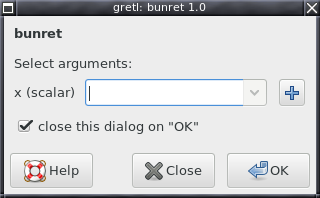
\includegraphics[width=0.4\textwidth]{figures/bunret-call}
\end{center}

Something may seem strange here: the function \texttt{bunret} returns
a bundle, but we're not seeing a slot to specify assignment of the
return value. But let's continue. If we type some value into the
\textsf{x} argument selector and click \textsf{OK} we get the window
shown in Figure~\ref{fig:bunret-window}, which gives two view of the
top part with two different menu buttons activated.

\begin{figure}[htbp]
\begin{center}
  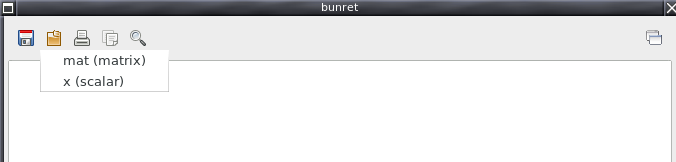
\includegraphics[width=0.75\textwidth]{figures/bunret-window1} \\
 \vspace{2ex}
  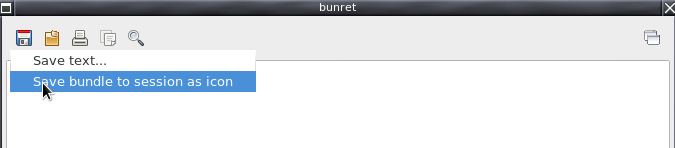
\includegraphics[width=0.75\textwidth]{figures/bunret-window2}
\end{center}
\caption{bunret output window}
\label{fig:bunret-window}
\end{figure}

So although we didn't get the option of assigning the bundle in the
function-call dialog, gretl has snagged the bundle on our behalf, and
will let us save its contents individually (upper picture), or the
whole thing ``as an icon'' (lower picture).

Another thing is noteworthy about the output window: its text area is
empty. That shouldn't be a surprise because the bunret function
doesn't print anything. Functions don't \textit{have} to print
anything, and gretl's built-functions generally do not, they just
return something useful. However, if a function is intended for GUI
use it probably should give some visible output, or in other words it
should be ``command-like.''

So let's revisit the package code. We could add suitable printing
commands within the \texttt{bunret} function itself, but for reasons
that will become apparent shortly, let's instead write a separate
printing function and add it to the package.
%
\begin{code}
function void bunret_print (bundle *b)
  printf "=== Hello from bunret_print ===\n\n"
  printf "The x member of %s is %g\n\n", argname(b), b.x
  printf "The matrix member is\n\n%10.3f\n", b.mat
end function
\end{code}
%
Having added this function (note, it should be public) we could then
call it from the main \texttt{bunret} function, but we won't do
that. Instead we'll select this function for the \texttt{bundle-print}
role in our package. In the GUI, you go to the ``Special functions''
tab under ``Extra properties'' to do that. And while we're at it,
since the package now has two public functions, we'll select
\texttt{bunret} for the \texttt{gui-main} role and in addition mark it
as ``no print,'' because it's not going to do any printing itself
(Figure~\ref{fig:special-funcs}).  In CLI mode, this means adding
three \textsf{spec} lines:
%
\begin{code}
gui-main = bunret
bundle-print = bunret_print
no-print = bunret
\end{code}

\begin{figure}[htbp]
\begin{center}
  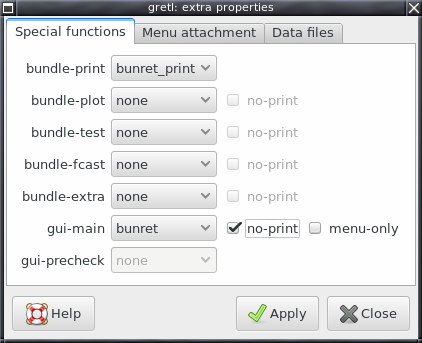
\includegraphics[width=0.5\textwidth]{figures/special-functions} \\
\end{center}
\caption{Selecting functions for special roles}
\label{fig:special-funcs}
\end{figure}

Here's how things will now work if we go back and call \texttt{bunret}
from the menu: gretl will snag the bundle as before, will notice that
this function is no-print, and will see if the \textsf{bunret} package
has a bundle-printer function. Since it does, it will call that
function on the bundle and put the result into the output window,
which will therefore no longer be blank. Your package's bundle window
is now somewhat like a gretl model window: it shows you some stuff and
allows you the possibility of saving some or all of it.

In addition, if the user decides to save your bundle ``as an icon,''
then subsequently double-clicking on the icon will again invoke the
bundle-print function, and re-create a window like the original one.

\tip{A word to the wise, in relation to the last Figure: clicking on
  Help in the ``Extra properties'' window brings up help text that is
  both specific to the active tab and reasonably complete. 'Nuff
  said.}

One more refinement here. This is a bit of a stretch when we're
looking at a little toy package, but you probably want to think about
both GUI users and users who may wish to call your package via
scripting. In the former case, as we've said, some visual feedback is
wanted, but in the latter case it should probably be optional
(assuming your function returns something).

Listing~\ref{ex:bunret} shows a modification of our toy package to
accommodate this. Hopefully it should be self-explanatory. We would
now make \dtkttt{GUI_bunret} the \texttt{gui-main} function and mark
it as \texttt{no-print}. Plain \texttt{bunret} (now intended for
script use) would not be ``no-print'' any more: it's silent by default
but the user can make it print by supplying a non-zero value for the
optional second argument. In CLI mode the relevant \textsf{spec} file
lines would be:

\begin{code}
public = GUI_bunret bunret bunret_print
gui-main = GUI_bunret
bundle-print = bunret_print
no-print = GUI_bunret
\end{code}

\begin{script}[htbp]
\caption{Toy package with GUI-specific function}
\label{ex:bunret}
\begin{scode}
function void bunret_print (bundle *b)
  printf "=== Hello from bunret_print ===\n\n"
  printf "The x member of %s is %g\n\n", argname(b), b.x
  printf "The matrix member is\n\n%10.3f\n", b.mat
end function

function bundle bunret (scalar x, bool verbose[0])
  bundle b
  b.x = x
  b.mat = I(3)*x
  if verbose
    bunret_print(&b)
  endif
  return b
end function

function bundle GUI_bunret (scalar x)
  return bunret(x)
end function
\end{scode}
\end{script}

\textit{Further reading}: For more on the special roles for functions
within packages see sections~\ref{sec:spec-gui} and
\ref{sec:spec-bundle}. In particular Section~\ref{sec:spec-bundle}
explains the requirements for a function to be a candidate for a
``bundle special'' role. For a discussion of how a real
package---\textsf{gig}, or GARCH in gretl, by Jack Lucchetti---does
this sort of thing see Section~4 of \cite{addons-bundles}, and for the
internals of \textsf{gig} itself, find \textsf{gig} in the browser for
packages on your local machine and select ``View
code.''\footnote{Depending on your platform, you may have to install
  gig first. Since \textsf{gig} is an official ``addon'' rather than a
  contributed package, installation is via the menu item ``Help, Check
  for addons'' in the gretl main window.} The GUI-related functions
are found towards the end of the code listing: start from
\dtkttt{gig_bundle_print} and \dtkttt{GUI_gig_plot}. You can also
open \textsf{gig} in the package editor and inspect its ``Extra
properties.'' The chapter titled ``User-defined functions'' in
\cite{GUG}, besides providing essential background for package
writers, details various refinements available when defining
parameters to a function for use in the GUI.

\subsection{Model-related packages}

The packages we've considered above offer ``top-level'' functionality,
in the sense that if they are to be shown in a menu they would
naturally appear somewhere in gretl's main window.

One can also write packages that do something interesting based on
data embedded in a gretl model---create a graph, run a test, do a
piece of analysis. Such functions (which may, but are not required to,
return bundles) have their proper place in menus on a gretl model
window, not the main menus.

Here's an overview of how such packages work.

\begin{enumerate}
\item The user estimates a model in the GUI and gretl constructs a
  window to show the output.
\item In the process of setting up the model-window menus, we check to
  see if any possibly relevant model-related packages are available.
\item If so, we run a ``pre-check'' (see below) to determine
  if the package can handle the particular sort of model in
  question.
\item If yes, we add a menu item for the package, and selecting this
  item pulls up a function call dialog for the package.
\item The function is then executed in an environment in which gretl's
  model-related accessors, such as \verb|$uhat|, target the displayed
  model.%$
\end{enumerate}

Let's consider this in some more detail.  First, how do we tell if any
possibly relevant packages are available? The mechanism here relies on
the package ``registry'' discussed in Section~\ref{sec:finer}. This
information is stored between gretl sessions in a file named
\texttt{packages.xml} in the user's gretl functions directory, which
is automatically read on start-up.

Second, how do we tell, for each model-related package, if it can
actually do something with a model that we're displaying? Two criteria
are relevant here, both under the control of the package author.

First there's the \texttt{model-requirement} field in the package
\textsf{spec} file. Valid entries for the field are the gretl
command-words corresponding to the various built-in estimators
(\cmd{ols}, \cmd{logit}, \cmd{mle} and so on). So for a function
specifically designed to handle logit models one could specify
\begin{verbatim}
model-requirement = logit
\end{verbatim}
(or make the equivalent selection under the ``Menu attachment'' tab of
the ``Extra properties'' window in the GUI package editor).

The above would imply that your package can handle all (and only)
logit models. In some cases you may want more fine-grained control
(e.g.\ you can handle both logit and probit, but only the binary
variants of these estimators). In that case you can use a second
mechanism, specifying a \texttt{gui-precheck} function
(Section~\ref{sec:spec-gui}).

This special function should not be included in the listing of public
interfaces; it is intended only for internal use by gretl. It must
take no arguments and must return a scalar, which is interpreted as an
error code (0 for OK, non-zero for not-OK). On execution it has access
to the \texttt{\$}-variables for the model in question. Among these is
the \texttt{\$command} accessor, which gives the command-word for the
estimator. So, for example, the pre-check function for a package which
targets binary logit and probit models might look like
Listing~\ref{code:precheck} (it could be written a good deal more
tersely, but the example shows the logic very explicitly).

\begin{script}[htbp]
\begin{code}
function scalar lpbin_precheck (void)
  string c = $command
  if c != "logit" && c != "probit"
    # can't handle this estimator
    return 1
  elif !isdummy($ylist[1])
    # logit/probit but non-binary, can't handle it
    return 1
  endif
  return 0
end function
\end{code}
\caption{GUI pre-check for binary logit or probit}
\label{code:precheck}
\end{script}
%$

Anything printed by a \texttt{gui-precheck} function goes to
\texttt{stderr}. This can be useful for debugging, but in the
``production'' version of a package the checker should operate
silently.

\subsection{Example: bandplot}
\label{sec:bandplot}

For a simple but idiomatic example of a model-related package, you
might take a look at \textsf{bandplot} (version 0.3 or higher), which
creates a plot displaying a confidence band for the effect of a
selected regressor in the context of a multiple regression.  In GUI
use, this package latches onto windows displaying models estimated via
OLS, attaching itself to the \textsf{Graphs} menu.

Here's the relevant part of \texttt{bandplot.spec}:

\begin{code}
description = Confidence band plot
min-version = 1.10.1
gui-main = GUI_bandplot
label = Confidence band plot
menu-attachment = MODELWIN/Graphs
model-requirement = ols
public = GUI_bandplot bandplot
no-print = GUI_bandplot bandplot
menu-only = GUI_bandplot
help = bandplot.help
gui-help = bpgui.help
\end{code}

The purpose of the optional \texttt{gui-help} keyword is to specify
help text to be presented in response to the \textsf{Help} button in a
dialog box. Note that in the online help for core gretl commands, a
distinction is made between text to be shown for scripting use and
text to be shown if the user clicks on \textsf{Help}. The former may
refer to option flags and arguments, the latter to buttons and
pull-down lists. The \texttt{gui-help} spec file item extends this
possibility to function packages. The string to the right of the
equals sign should give the name of a plain text (UTF-8) file
containing the GUI-specific help text. In the GUI you can edit or add
GUI help under ``Extra properties'' via a button in the ``Menu
attachment'' tab.

You may wonder, what happens if your package offers PDF documentation
but you also choose to give some \texttt{gui-help} text? Answer: when
the user clicks on \textsf{Help} in your GUI function-call dialog, she
will see the GUI help text in the first instance, but the window
showing this text will display a hyperlink to the PDF doc.

This package also illustrates some special GUI-related inflections in
the parameter listing for a user-defined function. Here's the
signature of \dtkttt{GUI_bandplot}, designed to be called from a
menu:
%
\begin{code}
function void GUI_bandplot (int xvar[$xlist] "x-axis variable",
     scalar conf[0.5:0.99:0.95:.01] "confidence level")
\end{code}
%$
Take the \texttt{conf} parameter first. Besides the usual
\texttt{[min:max:default]} fields for a scalar parameter, you can add
a fourth field to specify a ``step''. This is used only for
non-integer scalar parameters. To make the step value active, the
other three numerical fields must also be given.  In this case
\texttt{conf} will be represented by a ``spin-button'' with a minimum
of 0.5, a maximum of 0.99, an initial value of 0.95, and a
\textit{step} or increment of 0.01 when the button is clicked. The
step specifier is ignored outside the context of a GUI function-call
dialog. (This is not specific to model-related packages.)

The \texttt{xvar} parameter above illustrates a a facility specific to
model-related packages, and in particular to packages that target
models carrying a list of regressors: you can replace the usual
\texttt{[min:max:default]} fields for an integer-valued parameter with
a single special symbol, \texttt{[\$xlist]}.  The effect is that in a
GUI dialog the parameter is represented by a drop-down list showing
the names of the regressors (skipping the constant, if any). See
Figure~\ref{fig:bandplot-call}.

\begin{figure}[htbp]
\begin{center}
  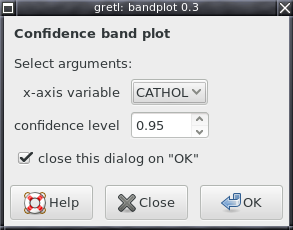
\includegraphics[width=0.4\textwidth]{figures/bandplot-call}
\end{center}
\caption{Call to \textsf{bandplot}, with special parameter-list
  inflections. Note the spin-button selector for \texttt{conf}
  (scalar) and the drop-down selector for \texttt{xvar} (int)
  as described in the text.}
\label{fig:bandplot-call}
\end{figure}

Based on the user's selection from the list, the argument is filled
out with the 1-based index of the position of the selected regressor
in the array of coefficients. For example, if the list of regressors
is \texttt{const x1 x2 x3} then the drop-down list will show
\textsf{x1}, \textsf{x2} and \textsf{x3}, and if the user selects
\textsf{x2} the value 3 will be given to \texttt{xvar}.

The idea is that if a package wants to single out a regressor, much
the most user-friendly way of conveying this to the user is to show a
list of names. There is no way that a package can arrange for this in
advance, so we want a means of signaling to gretl that the list should
be constructed at runtime, based on the particular model. But please
note, this special feature is not ignored in non-GUI use; it will
cause trouble. That's one reason why, as we saw in the spec file
extract above, \dtkttt{GUI_bandplot} is marked as \texttt{menu-only}.
Note that the \texttt{menu-only} attribute is also visible and
settable via the GUI package editor (Figure~\ref{fig:special-funcs}).

The other reason why \dtkttt{GUI_bandplot} is ``menu-only'' is
evident from the first line of code in the function, namely
%
\begin{code}
matrix b = $coeff
\end{code}
%$
This assumes that the model-related \texttt{\$}-accessors are primed
to refer to a valid model that, moreover, was estimated via
OLS. That's a safe assumption when coming off a model-window menu
(pre-screened by \texttt{model-requirement} and/or
\texttt{gui-precheck}), but in general it's not at all safe.

\subsection{No-print, once again}

We've already come across the \texttt{no-print} attribute of packaged
functions, but it's worth revisiting this in the context of functions
whose sole job is to produce a graph or plot of some kind (whether or
not they are model-related).

By default, when a packaged function is invoked via the GUI a window
is opened showing the command along with any printed output, but for
graph-only output such a window is superfluous and potentially
confusing.  You can suppress the text window by marking the function
in question as \texttt{no-print}. This applies to bandplot, but
would also apply to a main-window function whose job is just to
produce a plot.

\section{Publishing a package}
\label{sec:publish}

If you decide that you'd like to publish a package---that is, make it
available via the channels described in
Section~\ref{sec:acquire}---here's the procedure.

Preliminary: please double-check your package to ensure you have met
the requirements in Section~\ref{sec:common-req}. This will save
everyone's time.

\subsection{Uploading to the gretl server}

If you don't already have a login to the gretl package server, you
need to begin by creating one (please note, this is not the same thing
as a sourceforge login).\footnote{The URL will be given to you by
  gretl if you go to upload a package via the GUI, but for reference
  it's \url{http://gretl.sourceforge.net/apply/}.}

With a login in hand, there are two ways of uploading a package using
gretl. There's also a way of doing this independently of gretl, via
the shell, though this may not be convenient on MS Windows.

\textit{First gretl method}: open your package's \textsf{gfn} file in
the GUI package editor (you can get there via the package browser, or
via the main-window menu item ``File, Function packages, Edit
package'').  On clicking the \textsf{Save...} button you'll find an
item titled \textsf{Upload to server}. This will ask for your login
information then perform the upload. If your package specification is
such that a zip package is needed, gretl will take care of building an
up-to-date zip file and uploading that.

\textit{Second gretl method}: In the main gretl window, go to ``File,
Function packages, Upload package'' and choose the package to
upload. The file selection dialog will offer a choice of looking for
\textsf{gfn} or \textsf{zip} files. If you select a gfn file
and gretl determines that it's actually a zip file that needs
to be uploaded, it will attempt to build the zip package first.

\textit{Shell method}: Listing~\ref{ex:curl-upload} shows two shell
scripts, the first suitable for uploading a stand-alone gfn package
and the second for uploading a zip package. The first three lines of
each would, of course, have to be filled out appropriately for your
case.  These recipes rely on various components that are standard kit
on unix-type systems such as Linux and OS X: a Bourne-type shell; the
basic utility programs \app{basename} and \app{stat}; and the
\app{curl} program for doing the actual upload. See Appendix A for
some comments on doing this sort of thing on MS Windows.

\begin{script}[htbp]
  \centering
  \caption{Shell scripts for uploading packages}
  \label{ex:curl-upload}
\begin{scode}
# (1) simple gfn file variant
user=your_gretl_login
password=your_gretl_password
pkg=/path/to/your_package.gfn

savename=`basename $pkg`
curl -F login="${user}" -F pass="${password}" \
-F "pkg=@${pkg};filename=${savename};type=text/plain;charset=utf-8" \
https://gretl.sourceforge.net/cgi-bin/gretldata.cgi


# (2) zip file variant
user=your_gretl_login
password=your_gretl_password
pkg=/path/to/your_package.zip

bytes=`stat $pkg --printf="%s"`
savename=`basename $pkg`
echo "Uploading $pkg ($bytes bytes) as $savename ..."

curl -F login="${user}" -F pass="${password}" -F datasize="${bytes}" \
-F "pkg=@${pkg};filename=${savename};type=application/x-zip-compressed" \
https://gretl.sourceforge.net/cgi-bin/gretldata.cgi
\end{scode}
\end{script}
%$

\subsection{Staging}

When your package is successfully uploaded, it first goes into a
``staging'' area on the server, and the gretl developers who are
responsible for package-checking are notified by email. Before too
long, hopefully, you should hear from one of the developers, with a
response of Accept, Reject, or Revise and Resubmit.

Typically, packages will be rejected only if they are considered too
trivial, if it turns out that they're really just duplicating
functionality that's already available in gretl, or if they clearly
make no attempt to comply with the stated requirements (section
\ref{sec:common-req} again). Revise and Resubmit is a likely response
if your package seems basically sound but some improvements are
warranted.

Once your package is accepted it is moved out of staging and will
appear in the public package listing, both within gretl (``On
server'') and via the web interface.


\section{Maintaining a package}
\label{sec:maint}

Once you've uploaded a function package to the gretl server, hopefully
that won't be the end of the story: unless your package was totally
perfect on its first release (Ha!) you'll want to revisit it from time
to time with fixes or enhancements in mind.

The question arises: if your initial work was via the GUI, or via the
CLI, are you thereby committed to that mode of operation forever?
Certainly not. You can mix and match the two approaches, subject to
some basic requirements---although, if your package is truly complex,
we advise sticking with the commmand-line approach throughout.

\textit{Case 1}: You started via the GUI but you'd like to explore
maintaining your package by CLI means. Fine, you can disassemble your
\textsf{gfn} file by opening it in the GUI package editor, going to
the ``\textsf{Save...}'' button and selecting the options \textsf{Save
  as script} (decline the option to save the sample script along with
the packaged functions) and \textsf{Write spec file} (accept the
options to save the auxiliary files). This will create the source
files you need to rebuild your package by CLI means
(Section~\ref{sec:cli-build}).

\textit{Case 2}: You started via the CLI but you'd like to explore
maintaining your package by GUI means. Fine, you know that the
\texttt{makepkg} command will create a \textsf{gfn} file, which you can
then open in the GUI package editor to make changes. But you'd be wise
to use the ``\textsf{Save...}''-button options, as described above, to
keep your text-file sources in sync with your GUI-edited \textsf{gfn}
File, so that on the next revision it doesn't matter where you start.

\clearpage

\section*{Appendix A: The CLI on Windows}
\addcontentsline{toc}{section}{Appendix A: The CLI on Windows}

If you would like to use the command-line approach under MS Windows
you must make a preliminary choice: you can either
\begin{itemize}
\item stick to the native Windows way of doing things, or
\item install software which mimics a unix environment on Windows.
\end{itemize}

The first option is simpler, and probably best for most users. In this
case you will presumably be using \app{cmd.exe} as your shell. The
advantage of the second option is that it provides a much more
powerful and versatile shell, but if you just want to do the sorts of
things discussed in Section~\ref{sec:cli-build} \app{cmd.exe} is quite
adequate, with some help from a few small additions.  We offer some
more detail on the two options below.

\subsection*{Native Windows: cmd.exe}
\label{sec:cmd.exe}

This supports all the commands shown in Section~\ref{sec:cli-build}
except that the \app{make} utility is not present. But \app{make} for
Windows can be downloaded from the \textsf{GnuWin32} project on
sourceforge: see \url{http://gnuwin32.sf.net/packages/make.htm},
which provides a nice easy self-installer. You may also want
command-line \textsf{zip} and \textsf{unzip} from \textsf{GnuWin32}:
\url{http://gnuwin32.sf.net/packages/zip.htm}. (In both cases you
should select the option ``Complete package, except sources''.)

For anyone who's interested but not very familiar with
\textsf{cmd.exe}, a basic guide follows.  First, to get easy access to
the program go to the Windows desktop, right-click, and select New,
Shortcut. You'll be asked for the location of the target for the
shortcut. Most likely this should be
\begin{code}
c:\windows\system32\cmd.exe
\end{code}
(but you can browse to find it if need be). Click \textsf{Next}, give
the item a name, then \textsf{Finish}. Now right-click on the new
shortcut and select \textsf{Properties}: let's make this dude a bit
more functional.
\begin{enumerate}
\item Under the Shortcut tab, find ``Start in:''; this is the
  directory in which the shell will start and by default it's the
  directory that contains \textsf{cmd.exe}, which is \textit{not} a
  useful place to be for our purposes. Change it to
  \verb|%userprofile%| and it will open in
  your personal file space (make it something more specific if you
  like).
\item Under the Font tab, choose a decent TrueType font in place of
  the primitive raster default, for example Lucida Console at size 14.
\item Under the Layout tab, Window Size panel, give yourself a
  comfortable height for the window---say, 35 lines.
\item If you like, under the Colors tab select black for ``Screen
  text'' and white for ``Screen background'' to get a more modern
  look.
\end{enumerate}

Having fixed its properties, double-click on the new shortcut and you
should have a fairly decent-looking terminal window. The
\textsf{cmd.exe} window is sometimes called a ``DOS box.''  In fact it
has nothing to do with \textsf{DOS}---a long-obsolete 16-bit operating
system---but its default appearance is indeed a nasty blast from the
past. Hopefully we've improved on that.

A couple of other things are needed to get a usable shell: the
programs we'll be using have to be in the \texttt{PATH}, and we need a
decent text editor.

As regards the \texttt{PATH}, the gretl installer gives you the option
of adding the directory holding \textsf{gretl} and \textsf{gretlcli},
but that leaves the \textsf{GnuWin32} utilities. In \textsf{cmd.exe}
you can do something like
\begin{code}
PATH %PATH%;c:\program files\gnuwin32\bin
\end{code}
or on a 64-bit system
\begin{code}
PATH %PATH%;c:\program files (x86)\gnuwin32\bin
\end{code}
(with any adjustment needed for the specifics of your system). That
will work, but only for the duration of your current shell session.
You can add directories to the \texttt{PATH} permanently by diving
into ``Advanced system settings'' under Control Panel's ``System''
item, but there's another approach that may be preferable, namely
creating an AutoRun file for use with \textsf{cmd.exe}. This can
handle \texttt{PATH} as well as other things. Here's an example:
\begin{code}
@echo off
DOSKEY ls=dir /B
DOSKEY edit="C:\Program Files\Notepad++\notepad++.exe" $*
DOSKEY profile=notepad %USERPROFILE%\profile.cmd
PATH %PATH%;c:\program files (x86)\gnuwin32\bin
\end{code}
%
To activate this you would type the above (or a variant that works for
you) into \textsf{Notepad} and save it as \texttt{profile.cmd} in the
directory that corresponds to \texttt{\%USERPROFILE\%} for
you.\footnote{You can determine this by typing
  ``\verb|echo %USERPROFILE%|'' at the shell prompt (without the
  quotes).}  Then open the Registry editor, \textsf{regedit.exe}, and
navigate to HKEY\_CURRENT\_USER $\rightarrow$ Software $\rightarrow$
Microsoft $\rightarrow$ Command Processor.  Right-click in the
right-hand pane and select Add String Value: give the new entry the
name \textsf{AutoRun} and the value
\begin{code}
%USERPROFILE%\profile.cmd
\end{code}
This little file will then be run whenever you start \textsf{cmd.exe}.

The last line of \texttt{profile.cmd} puts the \textsf{GnuWin32}
programs into the path as promised. The other lines are just
illustrative of what's possible. \texttt{DOSKEY} establishes an alias,
so the first instance allows you to type \texttt{ls} to get a
directory listing, the second allows you to type, e.g., ``\texttt{edit
  Makefile}'' and have your Makefile opened by \textsf{Notepad++}, and
the third lets you type \texttt{profile} to open your shell AutoRun
file in Notepad in case it needs updating.

Speaking of \textsf{Notepad++}, unless you already have a personal
favorite text editor we strongly recommend using this program. The
\textsf{notepad.exe} supplied with Windows is a truly feeble piece of
software, easily confused by variant line-endings and inclined to hide
or misconstrue the true content of some text files. \textsf{Notepad++}
is very full-featured (it knows about the syntax of Makefiles, for
example) and also easy to use. It's free under GPL and available from
\url{http://notepad-plus-plus.org/}.

One more point: it's not always understood that you can launch GUI
programs from \textsf{cmd.exe}. We've alluded to one instance
above---typing \texttt{edit} at the command prompt to open a file in
\textsf{Notepad++}---but here's another that can be useful. Having
built a \textsf{gfn} file using \textsf{make} under the shell (see
Figure~\ref{fig:cmd-exe}) you can easily open it for inspection in the
gretl GUI with
%
\begin{code}
gretl mypkg.gfn
\end{code}
%
No need to mess with File Open dialogs since you're already in the
directory where \texttt{mypkg.gfn} is located.

\begin{figure}[htbp]
  \centering
  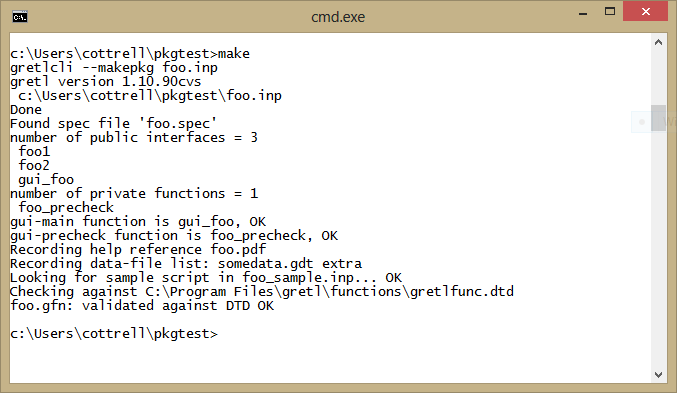
\includegraphics[width=0.75\textwidth]{figures/cmd-exe}
  \caption{Running make to build a gfn file on Windows}
  \label{fig:cmd-exe}
\end{figure}

\subsection*{Alternative: a unix-type shell}

There are two main packages which provide a unix-type shell on
Windows, \textsf{CygWin} and \textsf{MSYS2}. Both are likely to take
some getting used to for anyone unfamiliar with unix idioms.

We won't get into details here, but if you're interested in this
approach we recommend trying \textsf{MSYS2}. You can find an account
of this software in section 2 of ``Building gretl on MS Windows'' at
\url{https://gretl.sourceforge.net/winbuild/gretl-winbuild.pdf}.  For
building function packages (as opposed to building gretl itself)
you'll just need a few packages beyond a basic \textsf{MSYS2} install,
namely \texttt{make}, \texttt{zip} and \texttt{unzip}.

As a final note, even if you decide not to go ``all the way'' with
command-line methods, using \app{gretlcli} under either \app{cmd.exe}
or a unix-type shell is a nice way of exploiting certain gretl
features (output redirection, use of environment variables, etc.) and
may be quite useful in it own right.


\section*{Appendix B: Makefile basics}
\addcontentsline{toc}{section}{Appendix B: Makefile basics}

Here we give a brief summary of some aspects of Makefile syntax and
usage that are likely to be useful for package-building with gretl.

A Makefile has (or can have) two main parts: a first section which
defines variables, and a second section which defines rules. The
initial definition of variables is optional but it allows for
convenient shorthand when writing the rules, and also allows for easy
``portability'' (names can be changed in just one place).

Each Makefile rule has (up to) three components: a \textit{target};
zero or more \textit{dependencies}; and zero or more
\textit{instructions} for making the target. The target should be up
against the left margin and followed by a colon. The dependencies, if
any, should be listed following the colon. The instructions should be
listed directly below the target line, offset from the left margin
with a single tab character.\footnote{Explicit instructions are not
  always necessary, since \app{make} knows natively how to build
  certain kinds of targets. However, it doesn't know anything about
  gretl files.}

Listing~\ref{ex:make2} shows a variant of the simple Makefile from
Section~\ref{sec:using-make}, where we have added PDF documentation to
the package. In this example the initial section defines just one
variable, \texttt{PKG}. Note the special syntax for using the value of
a Makefile variable in the rules: the name of the variable must be
placed in parentheses, preceded by a dollar sign: \texttt{\$(PKG)}.

\begin{script}[htbp]
  \caption{Makefile for package with PDF documentation}
  \label{ex:make2}
\begin{scode}
PKG = mypkg

$(PKG).gfn: $(PKG).inp $(PKG).spec $(PKG)_sample.inp
	gretlcli --makepkg $(PKG).inp

$(PKG).pdf: $(PKG).tex
        pdflatex $<
        bibtex $(PKG)
        pdflatex $<
        pdflatex $<

$(PKG).zip: $(PKG).gfn $(PKG).pdf
	echo makepkg $(PKG).zip | gretlcli -b -

install: $(PKG).zip
	echo pkg install $(PKG).zip --local | gretlcli -b -

clean:
	rm -f $(PKG).gfn $(PKG).pdf $(PKG).zip
\end{scode}
\end{script}
%$

This Makefile specifies five targets. The first target (in this case,
the \textsf{gfn} file) is invoked if you simply type
``\texttt{make}''; to invoke the other targets you have to name them,
as in ``\texttt{make install}''.

If a target has no dependencies (like \texttt{clean} here) its
associated instructions are carried out unconditionally, so
``\texttt{make clean}'' will always attempt to delete the three files
that can be generated by \app{make}.  By the way, using the
\texttt{-f} (``force'') flag with the \texttt{rm} (``remove'') command
means that it will not seek confirmation, nor will it complain if the
file to be deleted doesn't actually exist.\footnote{This rule contain
  the only unix-specific idiom in the Makefile: under \texttt{cmd.exe}
  you would substitute \texttt{del} for \texttt{rm -f}.}

If the target of a Makefile rule is the name of a file, and the rule
has dependencies, then the instructions will be carried out if and
only if any of the dependencies were modified more recently than the
target file.  So ``\texttt{make}'' (with this Makefile) will simply
report
\begin{code}
make: 'mypkg.gfn' is up to date.
\end{code}
if the \textsf{gfn} file has already been built and nothing has
changed since among the files listed as dependencies.

On the other hand, if a target does not name a file, but is rather a
generic identifier such as \texttt{install}, it will get built
regardless. So ``\texttt{make install}'' in this example will always
(re-)install the package.

A couple of things should be noted about the \texttt{\$(PKG).pdf}
target: the \app{bibtex} instruction is wanted only if the \TeX{}
source contains a bibliography (which it probably should); and we use
here the built-in Makefile variable ``\texttt{\$<}'', which refers to
the first (or only) dependency of a rule.

Makefile rules are applied recursively---this is what makes \app{make}
so powerful. So, for example, ``\texttt{make install}'' will not fail
just because the \textsf{zip} file has not yet been built, so long as
the Makefile contains a recipe for building the latter (which of
course it does). By the same token, if you invoke the \texttt{install}
target when the \textsf{zip} file already exists, it will be checked
automatically for up-to-dateness and rebuilt if necessary---which also
means that the \textsf{gfn} and PDF files will be checked and possibly
rebuilt.

Any files specified as dependencies must either (a) feature as the
target of a rule, or (b) be provided as ``primitive'' inputs. In this
example the primitives are the \textsf{inp} file containing function
definitions, the \textsf{spec} file for the package, the sample
script, and the \TeX{} source for the documentation. Everything else
gets generated by \app{make}.

\chapter{Package specification details}
\label{chap:specfile}

Here we list and explain the usage of all the currently allowed
elements in the specification of a function package. We focus on the
\textsf{spec} file (from which a gretl function package may be
constructed by command-line means) but we also indicate the
representation of each specification element in the GUI package
editor.

We begin with a few general points on the \textsf{spec} file. Each
entry in this file takes the form

\texttt{keyword =} \textsl{value(s)}

Where multiple values are allowed, they should be separated by
spaces. An entry can be continued over more than one line if required,
using a trailing backslash (\verb+\+) as the continuation
character. Blank lines are ignored, as are lines beginning with the
hash mark (\texttt{\#}), which can be used to insert comments.  As
usual with gretl files, any non-ASCII characters should be UTF-8
encoded.

\section{Basic elements}
\label{sec:spec-basic}

The elements described in the section apply to all function packages,
whether or not they offer an interface specifically designed for
use via the gretl GUI and whether or not the main public function(s)
return a gretl bundle.

Elements in the first block below are all represented in the upper
panel of the GUI package editor window (see
Figure~\ref{fig:package_editor}).

\begin{description}

\item \texttt{author} (required): The name of the author of the
  package. Multiple names may be given, separated by ``and'', although
  note that this string may be truncated for presentation purposes in
  some contexts.

  \vbusage{} \verb|author = Riccardo "Jack" Lucchetti and Allin Cottrell|

\item \texttt{email} (required): The email address to which
  correspondence should be directed. Only one address should be given.

  \vbusage{} \verb|email = cottrell@wfu.edu|

\item \texttt{version} (required): The version number for the package
  release. This should be parseable as an integer or floating-point
  number (in the \textsf{C} locale). That is, it should contain only
  digits and at most one dot (\texttt{.}).

  \ttusage{version = 1.2}

\item \texttt{date} (required): The date on which the release was
  prepared, in ISO 8601 format, \textsf{YYYY-MM-DD}.

  \ttusage{date = 2015-03-28}

\item \texttt{description} (required): A short plain-text (UTF-8)
  string describing what the package does.

  \ttusage{description = logit/probit marginal effects}

\item \texttt{data-requirement} (optional): If this element is
  supplied, it must be one of the following strings:
  \texttt{no-data-ok}, \texttt{needs-time-series-data},
  \texttt{needs-qm-data} (meaning, quarterly or monthly time-series
  data), or \texttt{needs-panel-data}. Note that the \textit{default}
  requirement is that a dataset of some sort is in place (cross
  sectional, time series or panel). If your function does not take any
  series or list arguments (for example, it does something with
  matrices), you should use \texttt{no-data-ok} to indicate that a
  dataset is not required.

  \ttusage{data-requirement = needs-panel-data}

\item \texttt{tags} (required): Here you must specify at least one
  ``tag'' for your package based on the classification developed by
  the American Economic Association for use with the \textit{Journal
    of Economic Literature} (hence known as \textit{JEL tags}). This
  is to help users who are searching on the gretl server for packages
  that will perform some specific function. If you supply more than
  one tag, the tags should be separated by spaces. You can find a
  listing of the available tags at
  \url{http://gretl.sourceforge.net/cgi-bin/gretldata.cgi?opt=SHOW_TAGS}.

  \ttusage{tags = C13}

\item \texttt{min-version} (required): The identifier for the minimum
  gretl version on which the package is supported.  Ideally, this
  should truly be the first gretl version on which the package will
  run OK, but if in doubt it is preferable to specify a later version
  (users can always update) rather than an earlier one (on which the
  package might fail and give the user a bad impression). See
  Section~\ref{sec:versioning} for further details.

   \ttusage{min-version = 2018a}

\end{description}

The remaining ``basic'' elements are represented in the GUI
in various ways, as described below.

\begin{description}

\item \texttt{public} (required): A list of names of the public
  interfaces offered by the package.

  \vbusage{} \verb|public = GUI_lp_mfx lp_mfx_print mlogit_mfx \| \\
           \verb|                   mlogit_dpj_dx ordered_mfx |

  \textit{GUI}: this list can be accessed and modified via the
  \textsf{Add/Remove functions} button.

\item \texttt{sample-script} (required): the name of a hansl
   script (\texttt{.inp}) file that serves as exemplar for use
   of the package.

   \ttusage{sample-script = keane-mfx.inp}

   \textit{GUI}: access and edit via the \textsf{Edit sample script}
   button.

 \item \texttt{help} (required): The name of the file in which Help
   for this package can be found. This must be either a UTF-8 text
   file (with or without usage of markdown, see Section~\ref{sec:md})
   or a PDF file. The basename of the file should be the same as that
   of the package (as in \texttt{mypkg.gfn} and \texttt{mypkg.pdf}).
   The filename suffix must be \texttt{.pdf} for PDF or \texttt{.md}
   for markdown; for non-markdown text the suffix is not crucial but
   \texttt{.txt} is suggested.

  \vbusage{} \verb|help = lp-mfx_help.txt|

\end{description}

\section{GUI-related elements}
\label{sec:spec-gui}

The elements described in this section are applicable only if at least
one function in the package is designed to be called via gretl's
graphical interface. In the GUI package editor these elements are
shown in one or other tab of the the window that appears on clicking
the \textsf{Extra properties} button.

\begin{description}

\item \texttt{menu-attachment} (optional): Specifies a place within
  the gretl menu system under which the package should be made
  available. At present packages can attach to menus (a) in the main
  gretl window and (b) in windows displaying model estimates
  (only). In specifying a \texttt{menu-attachment} these are
  represented by the strings \texttt{MAINWIN} and \texttt{MODELWIN}
  respectively. The ``path'' to the entry for your package should
  start with one of these identifiers; this should be followed by one
  or more slash-separated elements, using the internal representation
  of the menu tree in \texttt{gretlmain.xml} or
  \texttt{gretlmodel.xml}---these XML UI files can be found in the
  gretl source package or in git.\footnote{See
    \url{http://sourceforge.net/p/gretl/git/ci/master/tree/gui/}.}

  \ttusage{menu-attachment = MODELWIN/Analysis}

\item \texttt{label} (conditionally required): A very short string
  that can be displayed in a GUI menu. This is relevant only if the
  package specifies a \texttt{menu-attachment}, in which case it is
  required.

  \ttusage{label = Marginal effects}

\item \texttt{gui-main} (optional): This entry is relevant only if a
  package offers more than one public interface. Its effect is to
  select one particular interface when a user accesses the function
  package via the gretl GUI (other public interfaces can be selected
  via the command line if the user so chooses). If a package offers
  multiple public interfaces and \texttt{gui-main} is \textit{not}
  specified, the user will be given a choice of interfaces whenever he
  or she calls the package. (If a package offers only one public
  interface, we can think of this as implicitly its ``gui-main''.)

  \vbusage{} \verb|gui-main = GUI_lp_mfx|

\item \texttt{gui-help} (optional): The name of a UTF-8 file
  containing GUI-specific help text, to be shown when the user clicks
  on \textsf{Help} in a dialog box representing the package. Such text
  may make reference to buttons, pull-down lists and the like rather
  than using language appropriate to command-line usage. To edit this
  text in the GUI package editor click on \textsf{Extra properties},
  select the \textsf{Menu attachment} tab and click on the \textsf{GUI
    help text} button.

  \ttusage{gui-help = bpgui.help}

\item \texttt{menu-only} (optional): A list of public interfaces (in
  practice, probably only one) that are specifically designed to be
  called from a suitable GUI menu and that should \textit{not} be
  offered via the browser for installed packages. If any function
  falls in this category it's likely to be the one designated as
  \texttt{gui-main}.

  \vbusage{} \verb|menu-only = GUI_lp_mfx|

\item \texttt{model-requirement} (optional): When the ``gui-main''
  function of a package is designed to be called from a menu in a
  gretl model-output window, this element can be used to indicate that
  only models of a certain type are supported (and therefore the
  package will shown only for such models).  The right-hand value
  should be the gretl command-word corresponding to the supported
  estimator. See also \texttt{gui-precheck}.

  \ttusage{model-requirement = tobit}

\item \texttt{gui-precheck} (optional): Applies only when a
  \texttt{menu-attachment} is specified. This element identifies a
  function to be called to check whether the package is supported in
  context.  It offers a more flexible testing mechanism than
  \texttt{model-requirement}.

  The \texttt{gui-precheck} function should not be included in the
  listing of public interfaces; it is intended only for internal use
  by gretl. It must take no arguments and must return a scalar. On
  execution it has access to all the \texttt{\$}-accessors for the
  model in question. On this basis the function should return 0 if the
  model is supported, non-zero otherwise.

  \vbusage{} \verb|gui-precheck = lp_mfx_precheck|

\item \texttt{list-maker} (optional): Applies only when a model-window
  \texttt{menu-attachment} is specified. This element identifies a
  function to be called to construct a list of series bearing some
  specific relationship to the gretl model which the package
  ``targets,'' from which the user is then expected to select a
  member. This is a generalization of the \texttt{\$xlist} mechanism
  described in Section~\ref{sec:bandplot} above, and is best explained
  by example. In the \textsf{exogtest} package the designated
  \texttt{list-maker} function reads as follows:
\begin{code}
function list exogtest_listmaker (void)
  bundle m = $model
  list L = m.xlist - m.instlist
  if nelem(L) == 0
    funcerr "No endogenous regressors were found"
  endif
  return L
end function
\end{code}
  %
  This function constructs a list of endogenous regressors from a
  model estimated via gretl's \texttt{tsls} command (details of which
  are presumed to be available as members of the \texttt{\$model}
  bundle). This then provides an automatic listing of candidate
  arguments for the \texttt{xvar} parameter to the package's
  \dtkttt{GUI_exogtest} function, the signature of which is
\begin{code}
function bundle GUI_exogtest (int xvar[$mylist] "regressor to test")
\end{code}
  %$
  The dummy default value of \texttt{\$mylist} is understood by gretl
  to mean the user's selection from the list returned by the
  \texttt{list-maker} function.

  Note that the \texttt{list-maker} function must take no arguments
  (but can assume access to \texttt{\$model}) and must return a list
  (or fail with an error message if no suitable list members are
  available). It should be a function private to the package.

  \ttusage{list-maker = exogtest\_listmaker}

\item \texttt{ui-maker} (optional): This element allows a package
  writer control over certain aspects of the dialog box shown when the
  \texttt{gui-main} function of a package is called.  Control is
  exercised via a private function which returns a bundle, holding a
  sub-bundle for each parameter to be inflected. The \texttt{ui-maker}
  is called internally when the relevant dialog box is to be shown,
  and on successful execution the directives in the returned bundle
  are followed. Since this functionality is somewhat complex, its
  details are set out separately in Section~\ref{sec:ui-maker} below.

  \ttusage{ui-maker = rf\_ui\_maker}

\item \texttt{no-print} (optional): A list of public interfaces that
  are not designed to print anything.  Consider, for example, a
  package whose job is to produce a special graph based on model data.
  By default, when a packaged function is invoked via the GUI a window
  is opened showing the command along with any printed output, but for
  graph-only output such a window is superfluous and potentially
  confusing. You can suppress the text output window by adding such a
  function to the \texttt{no-print} list.

  \ttusage{no-print = foo\_plot}

\end{description}

\section{More on the GUI: ui-maker}
\label{sec:ui-maker}

The basic idea of the \texttt{ui-maker} function has been introduced
above; in this section we delve into the details.  First, note that
the private function that supports this functionality must take no
arguments, and must return a bundle containing one or more
sub-bundles, each identified by the name of a parameter whose GUI
representation the author wishes to inflect, and each of which
contains one or more special keys corresponding to recognized
directives. So in outline such a function should look something like
this:

\begin{code}
function bundle my_uimaker (void)
    bundle ret
    #
    # add parameter-specific sub-bundles to @ret here
    #
    return ret
end function
\end{code}

Also note that in the graphical interface the parameter list for a
function translates into an array of widgets by means of which
arguments corresponding to the parameters are set. This is a
one-to-one mapping so you can refer to particular widgets by the name
of the corresponding parameter.

The aspects of the GUI that a function writer can control, or at least
inflect, via \texttt{ui-maker} fall into three categories: conditional
sensitivity of argument widgets, run-time determination of the
minimum, maximum and/or default values for arguments, and restrictions
relating to list arguments (lists of series, that is). We go into each
of these below. For concreteness, we'll assume that the
\texttt{ui-maker} returns a bundle named \texttt{ret}, as in the
example above (though you're to choose the name yourself).

\subsection{Conditional sensitivity}

The widget for a given parameter---denoted by \textsf{W}$_i$, where
$i$ indicates its place in the parameter list---can be made sensitive
or insensitive (``grayed out'') conditional on the state of the widget
representing a prior parameter, \textsf{W}$_j$, $j<i$. This is
achieved via a string under the key \texttt{depends} in the sub-bundle
for \textsf{W}$_i$.  In the simplest case this is just the name of a
prior boolean parameter, where \textsf{W}$_j$ takes the form of a
check-box. Suppose we want the widget for a parameter \texttt{baz} to
be shown as sensitive if and only if the check-box for a parameter
\texttt{foo} is checked. Then this statement in the \texttt{ui-maker}
would do the job:
\begin{code}
ret.baz = _(depends = "foo")
\end{code}

Alternatively, \texttt{depends} may take the form
\textsl{name}\,\texttt{cmp}\,\textsl{value}, where \textsl{name} is
the name of parameter $j$, \textsl{value} is an integer indicating the
state of \textsf{W}$_j$ and \texttt{cmp} is a `comparator':
``\texttt{=}'' (or ``\texttt{==}'') for equality; ``\texttt{!=}'' for
inequality; ``\texttt{<}'' and ``\texttt{>}'' for less than or greater
than, respectively.

If \textsf{W}$_j$ is a check box only the equality comparator is
supported, but this allows for for inverse dependency. Given
\begin{code}
ret.baz = _(depends = "foo=0")
\end{code}
the widget for \texttt{baz} will be sensitive if and only if the box
for parameter \texttt{foo} is \textit{not} checked.

The extended case also allows for dependency on a ``combo box''
holding a pull-down list of options. Suppose we have a parameter named
\texttt{bar}, represented thus in the signature of the function in
question:
\begin{code}
int bar[0:2:0] "some option" {"none", "basic", "advanced"}
\end{code}
Then we can make the sensitivity of parameter \texttt{baz} conditional
on the state of \texttt{bar} in various ways:
\begin{code}
# sensitive if option 2 for bar is selected
ret.baz = _(depends = "bar=2")
# sensitive if any option but 0 is selected
ret.baz = _(depends = "bar>0")
# sensitive if an option lower than 2 is selected
ret.baz = _(depends = "bar<2")
\end{code}
Note that the \textsl{value} to the right of the comparator refers to
the numbering in the specification of \texttt{bar}. If the three
option values were given as \texttt{[1:3:1]} instead of
\texttt{[0:2:0]}, the \texttt{depends} condition would have to be
modified accordingly.

\subsection{Run-time limits and defaults}

This facility is relevant if your package requires that a dataset be
in place. In that case your \texttt{ui-maker} function will have
access to all the usual dataset-related accessors; limits and/or
default values can then be conditioned on the characteristics of the
data. This is supported for parameters of type \texttt{int} and
\texttt{scalar}, via the keys \texttt{minimum}, \texttt{maximum} and
\texttt{default}. In each case the value of the bundle element should
be a string: a valid hansl expression which yields a scalar value.

For example, suppose that your function has a parameter \texttt{n}
whose value should be no greater than 20 percent of the current sample
size. Then you could include the following statement in your
\texttt{ui-maker} (where \texttt{ret} is the bundle to be returned):

\begin{code}
ret.n = _(maximum="floor(0.2*$nobs)")
\end{code}

If in addition you want the default value to equal the maximum, you
could substitute
\begin{code}
string maxstr = "floor(0.2*$nobs)"
ret.n = _(maximum=maxstr, default=maxstr)
\end{code}

And of course you could add a data-dependent minimum value if that's
wanted.

\subsection{Restrictions on list arguments}

A parameter calling for a list of series can be inflected in any of
three ways, via the following keys.

\begin{itemize}
\item \dtkttt{list_no_singleton} is a boolean, with a default value
  of 0, meaning that it's acceptable for a list to have a single
  member. If you want to ensure that a particular list contains more
  than one series, give a value of 1 for this key.
\item \dtkttt{list_no_const} is also a boolean with a default value
  of 0, meaning that it's acceptable for a list to contain the
  automatic \texttt{const} series. To prevent inclusion of
  \texttt{const} give a value of 1 for this key.
\item \dtkttt{list_exclude} requires a string value, the name of a
  parameter of type series. The effect is to ensure that if a given
  series has been selected for that parameter it should not be shown
  as a candidate for inclusion in the list in question.
\end{itemize}

To illustrate, suppose a function has a series parameter \texttt{y}
and a list parameter \texttt{X}, with three conditions placed on
\texttt{X}: it contains more than one series, does not contain
\texttt{const}, and does not contain the series selected as
\texttt{y}. Then the following would do the job:
\begin{code}
ret.X = _(list_no_singleton=1, list_no_const=1, list_exclude="y")
\end{code}

These keywords can also be given in a shorter form, omitting the
\dtkttt{list_} prefix, but the more explicit long version is
recommended for clarity.

\subsection{Real-world examples}

Here we give some ``live'' illustrations of \texttt{ui-maker}
functionality based on current function packages.

First take \textsf{cffilt} by Jack Lucchetti, which computes the
Christiano--Fitzgerald (CF) band-pass filter. This package requires
time-series data. The usual application of the CF filter is to extract
information at business-cycle frequencies from annual, quarterly or
monthly macroeconomic data, in which case suitable defaults for the
lower and upper limits for the pass band (minimum and maximum number
of periods) can easily be calculated based on the data
frequency. However, the filter could also be used on data observed at
other frequencies; then it's not so clear what the pass band should
look like.

In the \texttt{gui-main} function of \textsf{cffilt} the minimum and
maximum periods take the form of integer parameters \texttt{pl} and
\texttt{pu}, which are given purely notional default values of 2 and
3, respectively. Problem: how to provide sensible default values at
run time, when possible? The solution looks something like this:

\begin{code}
function bundle cf_ui_maker (void)
    bundle ret
    if $pd == 1 || $pd == 4 || $pd == 12
        # annual, quarterly or monthly
        ret.pl = _(default="ceil(1.5*$pd)")
        ret.pu = _(default="8*$pd")
    endif
    return ret
end function
\end{code}

Note that if the data are of non-standard frequency, the bundle
returned by \dtkttt{cf_ui_maker} will be empty. That's OK, it just
means the default values for \texttt{pl} and \texttt{pu} will remain
at those set in the \texttt{gui-main} function.

For a second example, take a look at the (slightly simplified)
signature of the \texttt{gui-main} for \textsf{random\_forest} by
Allin Cottrell, which provides a gretl interface to the \textsf{R}
package \textsf{randomForest}:
\begin{code}
function bundle GUI_rf (series y "dependent variable",
   list X "independent variables",
   int n_train[50::] "training observations",
   bool use_seed[0] "set random seed",
   int seed[0:2147483647:1234567])
\end{code}

Consider the parameters \texttt{y} and \texttt{X}. Obviously, we don't
want the series that's selected as the dependent variable to be
included in the list of independent variables. Plus, in this
machine-learning context it doesn't make sense to have a single
independent variable, nor to include a constant. So here's a case in
point for the full form of the list-restriction mechanism described
above.  The \texttt{ui-maker} for this package (still assuming the
return value is called \texttt{ret}) includes
\begin{code}
ret.X = _(list_no_singleton=1, list_no_const=1, list_exclude="y")
\end{code}

Now focus on \dtkttt{n_train}, the number of observations to be used
for training. The signature above specifies a minimum of 50 but leaves
the maximum and default values undetermined. The \texttt{ui-maker} can
then fill in these values depending on the number of observations,
something like:
\begin{code}
maxstr = "ceil(0.9*$nobs)"
defstr = "ceil(0.65*$nobs)"
ret.n_train = _(maximum=maxstr, default=defstr)
\end{code}

Finally, consider the \dtkttt{use_seed} and \texttt{seed}
parameters. The Random Forest algorithm, as the name implies, employs
randomization. Setting a known seed for the random number generator
will give reproducible results, otherwise results may differ somewhat
on each run. The seed parameter is relevant only if the user wants to
set a seed, so this is a case for \texttt{depends} in the
\texttt{ui-maker}:
\begin{code}
ret.seed = _(depends="use_seed")
\end{code}
Unless the user checks the \dtkttt{use_seed} box, the \texttt{seed}
widget will remain grayed out.

\section{Bundle-related elements}
\label{sec:spec-bundle}

The elements described below are applicable only if at least one
public function in the package returns a bundle. In the GUI package
editor these appear under the \textsf{Special functions} tab in the
\textsf{Extra properties} window.

\begin{description}

\item \texttt{bundle-print} (optional): Identifies a given function that can
  be used to print the content of a bundle produced by the package.

  \vbusage{} \verb|bundle-print = oddsratios_print|

\item \texttt{bundle-plot} (optional): Identifies a given function that can
  be used to produce some sort of plot or graph using the content of a
  bundle produced by the package.

  \vbusage{} \verb|bundle-plot = SF_Plot|

\item \texttt{bundle-fcast} (optional): Identifies a function that
  generates a forecast based on a bundle's content.

  \vbusage{} \verb|bundle-fcast = regls_fcast|

\item \texttt{plot-precheck} (optional): Relevant only if the package
  includes a \texttt{bundle-plot} function. Identifies a function that
  signals whether a plot is actually available, conditional on the
  content of the bundle.

  \vbusage{} \verb|plot-precheck = regls_plot_check|

\end{description}

Functions selected for the special bundle-related roles may be public (if it
makes sense to allow users to call them directly) or private (if they're
designed to be called only via GUI hooks). In either case they must conform
to certain rules, as follows.
\begin{itemize}
\item In all cases the first argument must be a bundle-pointer.
\item In the case of \texttt{bundle-fcast} this is followed by two
  mandatory integer arguments giving the start and end of the sample
  range for the forecast. In other cases the second argument, if
  present, must be an \texttt{int} that controls the function's
  behavior in some way, and it must have a specified default value.
\item Any further arguments must have default values (meaning that
  they can be omitted).
\end{itemize}

Taking the \textsf{gig} package as an example, we have:
%
\begin{code}
  function void gig_bundle_print(bundle *model)
\end{code}
%
and
%
\begin{code}
function void GUI_gig_plot(bundle *model, int ptype[0:2:0] \
                           "Plot type" {"Time series", "Density", "Forecast"})
\end{code}

That is, \textsf{gig}'s \texttt{bundle-print} function has no options,
but its \texttt{bundle-plot} function has a control parameter
\texttt{ptype}. Note how this parameter is set up: it has a minimum
value of 0 and a maximum of 2 (these options could be extended), and 0
is the default. Further, the parameter is given a name for display in
the GUI, ``Plot type'', and it also has strings---``Time series'',
``Density'' and ``Forecast''---associated with its three possible
numerical values. The latter strings will be used to populate a menu
on the window displaying a \textsf{gig} bundle
(see Figure~\ref{fig:gig-plot-menu}).
\vspace{1ex}

\begin{figure}[htbp]
  \begin{center}
  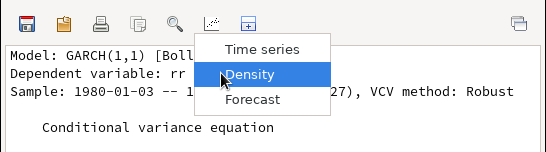
\includegraphics[scale=0.7]{figures/gig_plot_menu.png}
  \caption{\texttt{gig} plot menu: the menu pops up from the plot
    toolbar button behind it.}
  \label{fig:gig-plot-menu}
  \end{center}
\end{figure}

Now it may be that the availability of plotting options (if any)
depends on the parameters with which the bundle in question was
created. For example, if producing a forecast is an optional extra
that has not been selected, a forecast plot should not be shown as a
``live'' option in the bundle window. This sort of case can be handled
by a \texttt{plot-precheck} function. There are two cases to consider.
\begin{itemize}
\item The \texttt{bundle-plot} function supports a single type of
  plot. In this case we'll say $p = 1$.
\item The \texttt{bundle-plot} function offers $p > 1$ options, with
  associated strings.
\end{itemize}
In each case \texttt{plot-precheck} must return a binary $p$-vector,
with 1s indicating options that are available given the bundle content
and 0s indicating unavailable options. The effect in the GUI is as
follows. Let $z$ denotes the number of 0s in the vector returned by
\texttt{plot-precheck}. Then
\begin{itemize}
\item if $z = p$ no plots are available and the plot toolbar button
  itself is insensitive (can't be clicked).
\item if $0 < z < p$ the button is sensitive but the unavailable menu
  item are shown as ``grayed out''.
\end{itemize}

\section{Extra elements}
\label{sec:spec-extra}

At present there are five spec file entries in this category; in the
GUI package editor they appear in the \textsf{Extra properties} window
under the tabs \textsf{Data files}, \textsf{Dependencies}, and
\textsf{Menu attachment}.

\begin{description}

\item \texttt{data-files}: Specifies an extra file or subdirectory
  that should be included in the package. Use of this option is valid
  only if the package takes the form of a zipfile. If just one extra
  file is to be included you may give its name as the parameter to
  \texttt{data-files} (as in the example below); if several extra
  files are to be packaged, put them into a subdirectory and give its
  name as parameter. See chapter~\ref{chap:zipfile} for examples, and
  in particular Section~\ref{sec:HIP} for the special meaning of
  including a subdirectory named \texttt{examples}.

  \ttusage{data-files = special.gdt}

\item \texttt{depends}: Specifies one or more packages upon which the
  given package depends. This information should be added if the
  package calls functions that reside in other packages.  Use of this
  option ensures that when your package is loaded, any dependencies
  are also loaded.  For example, there's a package named
  \texttt{extra} which provides various utility functions that are not
  available as gretl built-ins.  If your package uses functions from
  \texttt{extra} you should include the following line in its spec
  file.

  \ttusage{depends = extra}

\item \texttt{provider}: This should be used if your package requires
  access to the \textit{private} functions of another package, a
  particularly close form of dependency. Only one package can be
  specified in this way.  In the GUI this feature is represented by a
  check box against the first entry under the \textsf{Dependencies}
  tab. In the spec file, specifying a package as provider
  automatically includes it as a dependency.

  \ttusage{provider = extra}

\item \texttt{wants-data-access}: In some cases your package may need
  to read data outside of the active sample range. This could be
  pre-sample initial values in a dynamic model, or it could be
  post-sample values of exogenous regressors used for out-of-sample
  (conditional) forecasting.  But since a user-written hansl function
  is normally restricted to the incoming sample specified by the
  caller of the function, this would not be possible. In such
  situations, your package should specify this switch, and if upon
  execution the gretl user agrees, your relevant packaged function may
  use the \texttt{smpl} command to reset the active sample inside the
  function even beyond the incoming limits. (The original sample will
  be restored when exiting the function, as always.) In the GUI
  package editor this item appears under \textsf{Menu attachment}.

  \ttusage{wants-data-access = true}

\item \texttt{R-depends}: This should be used if your package depends
  on \textsf{R} for its functionality. You should give an \textsf{R}
  version with which the package is known to work, along with the
  names and known-good version numbers of any \textsf{R} packages it
  requires. The example below might be suitable for a package that
  requires \textsf{R} and its \textsf{glmnet} package. Multiple
  elements should be separated by spaces

  \ttusage{R-depends = R 3.5.3 glmnet 2.0-18}

\item \texttt{R-setup}: This is specific to packages that call upon
  \textsf{R}. The required parameter is the name of a private hansl
  function, whose role is to define an \textsf{R} function. The hansl
  function should take no arguments and should not return anything
  (that is, be of type \texttt{void}). It should just be a thin
  wrapper over a gretl \texttt{foreign} block, as illustrated in
  Listing~\ref{ex:rsetup}.

  This mechanism depends on access to the \textsf{R} shared library,
  which will usually be available when \textsf{R} is installed. The
  idea is that the \textsf{R} function in question is ``registered''
  with the \textsf{R} library when your package is loaded, and can
  thereafter be called---with the prefix ``\texttt{R.}''---as if were
  a native gretl function, avoiding the need for further use of a
  \texttt{foreign} block. In relation to Listing~\ref{ex:rsetup}, once
  \texttt{foo} is registered with \textsf{R}, hansl code in your
  package can call \texttt{R:foo} (with suitable arguments, of course)
  and retrieve whetever it returns, without need for further use of
  gretl's \texttt{foreign} apparatus.

  To gain a fuller understanding of this facility, please refer to
  Chapter 44 of the \GUG, in particular section 44.7, ``Further use of
  the R library''. Here we'll just note that when a package includes
  an \texttt{R-setup} function it is tested for applicability when the
  package is first loaded. If the \textsf{R} library cannot be found
  or the \textsf{R} code to define a function is not successfully
  executed, the problem should be quickly apparent.

  \ttusage{R-setup = foo\_setup}

\begin{script}[htbp]
  \caption{Skeleton of an \texttt{R-setup} function}
  \label{ex:rsetup}
\begin{code}
   function void foo_setup (void)
      foreign language=R --quiet
      foo <- function(<args>) {
         # R code goes here
      }
      end foreign
   end function
\end{code}
\end{script}

The \textsf{random\_forest} package for gretl, mentioned in
Section~\ref{sec:ui-maker} above, uses the \texttt{R-setup} apparatus.
A hansl function named \dtkttt{rf_setup} defines an \textsf{R}
function named \texttt{randforest}, which is then called as
\texttt{R.randforest} elsewhere in the package code. The relevant code
can be inspected at
\url{https://github.com/AllinCottrell/function_packages/blob/main/rf-ng/rf_main.inp}.

\end{description}

\section{A note on gretl versioning}
\label{sec:versioning}

Since 2015 gretl version identifiers have taken the form ``year of
release plus sequential letter''---as in \texttt{2018a},
\texttt{2018b} and so on---and this form should be used when
specifying the minimum gretl version required by a package via its
\texttt{spec} file. Note that you can consult the gretl ChangeLog
(\url{http://gretl.sourceforge.net/ChangeLog.html}) to determine when
commands or functions of interest were introduced. A reasonable policy
would be to specify a minimum gretl version dating from, say, two or
three years prior to the writing of your package, unless the package
depends on more recently added functionality.

\chapter{Zip package details}
\label{chap:zipfile}

\section{Basic specification}

At minimum, a zip package must contain a top-level directory with the
same name as the package itself, and this directory must contain the
\texttt{gfn} file. Suppose the name of the package is \textsf{mypkg};
in that case the minimal zipfile looks like this (as shown by the
\textsf{unzip} program with its \texttt{-l} option to list the
contents of an archive):

\begin{code}
Archive:  mypkg.zip
  Length      Date    Time    Name
---------  ---------- -----   ----
        0  2015-06-07 10:54   mypkg/
    10708  2015-06-07 10:54   mypkg/mypkg.gfn
---------                     -------
    10708                     2 files
\end{code}

There would be little point in creating a package with just the
content shown above; the advantage of the zipfile format lies in the
possibility of including extra materials that cannot be stuffed into
a \texttt{gfn} file. Such materials fall into four main categories:

\begin{itemize}
\item PDF documentation. This should take the form of a pdf file with
  the same basename as the package, included in the top-level package
  directory. Thus, to continue the example above, the directory
  \texttt{mypkg} might contain \texttt{mypkg.pdf} as well as
  \texttt{mypkg.gfn}.
\item Data to support a sample script. This answers the case where a
  package author wishes to use specific data, not present in the gretl
  distribution, with his or her sample script. For example, the
  \textsf{almonreg} package contains the datafile \texttt{almon.gdt}
  to permit replication of Shirley Almon's original modeling.
\item Data for internal use. For example, gretl matrix files
  containing tables of critical value for some hypothesis test
  implemented by the package.
\item Extra examples: scripts and/or data files that go beyond the
  required sample script to give users a full sense of the scope and
  usage of a complex package.
\end{itemize}

\section{Example: \textsf{almonreg}}

Here's a fairly simple real case, the \textsf{almonreg} package:

\begin{code}
Archive:  almonreg.zip
  Length      Date    Time    Name
---------  ---------- -----   ----
        0  02-12-2015 13:27   almonreg/
    55861  02-12-2015 13:27   almonreg/almonreg.pdf
     4409  02-12-2015 13:27   almonreg/almonreg.gfn
     1969  02-12-2015 13:27   almonreg/almon.gdt
---------                     -------
    62239                     4 files
\end{code}

The relevant portion of the \textsf{almonreg} spec file, calling for
inclusion of the PDF and gdt files, reads thus:

\begin{code}
help = almonreg.pdf
data-files = almon.gdt
\end{code}

Note that when the \textsf{almonreg} sample script opens the data file
\texttt{almon.gdt} it must employ the \option{frompkg} option to tell
gretl where to find the file:

\begin{code}
open almon.gdt --frompkg=almonreg
\end{code}

\section{Example: \textsf{GHegy}}

Another illustration: Ignacio D\'iaz-Emparanza's \textsf{GHegy}
package (abbreviated):
%
\begin{code}
Archive:  GHegy.zip
  Length      Date    Time    Name
---------  ---------- -----   ----
        0  2015-03-12 13:51   GHegy/
    18610  2015-03-12 13:51   GHegy/GHegy.gfn
        0  2015-03-12 13:51   GHegy/coeffs/
    52960  2015-03-12 13:51   GHegy/coeffs/CFt_c_fijo.mat.gz
    53276  2015-03-12 13:51   GHegy/coeffs/CFt_cD_fijo.mat.gz
    42990  2015-03-12 13:51   GHegy/coeffs/Ct2_c_BIC.mat.gz
    ...    ...                ...
---------                     -------
  3798063                     83 files
\end{code}

In this instance we don't have PDF documentation, but we do have a
large number of gzipped gretl matrix files, holding response-surface
coefficients by means of which the package is able to compute
$P$-values for the HEGY seasonal unit-root test. The relevant
spec file clause is
%
\begin{code}
data-files = coeffs
\end{code}
%
Note that putting \texttt{coeffs} (the name of a directory) into the
data-files list ensures that all the contents of this directory will
be included in the zip package. At run time \textsf{GHegy} can access
its matrix files using the accessor variable
\verb|$pkgdir|, which will expand to the appropriate
platform-dependent path, as in
%
\begin{code}
string matname = sprintf("%s/coeffs/CFt_c_fijo.mat.gz", $pkgdir)
matrix C = mread(matname)
\end{code}

\section{Example: \textsf{HIP}}
\label{sec:HIP}

Our final illustration is the \textsf{HIP} package (which now has
official ``addon'' status), written by Jack Lucchetti and Claudia
Pigini. Looking in the zipfile we see:

\begin{code}
Archive:  HIP.zip
  Length      Date    Time    Name
---------  ---------- -----   ----
        0  03-19-2015 19:58   HIP/
        0  03-19-2015 19:58   HIP/examples/
    75210  03-19-2015 19:58   HIP/examples/camtriv_chap14.gdtb
      657  03-19-2015 19:58   HIP/examples/camtriv_chap14.inp
     1941  03-19-2015 19:58   HIP/examples/MonteCarlo.inp
   383278  03-19-2015 19:58   HIP/HIP.pdf
    27691  03-19-2015 19:58   HIP/HIP.gfn
---------                     -------
   488777                     7 files
\end{code}

We have PDF documentation plus an \texttt{examples} directory. The
latter is special: if a zip package contains a directory named
\texttt{examples} (\textit{exactly} that, in English and all lower
case), then in the GUI function package browser the ``Resources...''
button (open folder icon) and menu item become active. Selecting this
item opens a file dialog pointing at the examples directory, from
which you can open any scripts or datafiles that are provided. These
are intended to supplement the required sample script.


\bibliography{gretl}

\end{document}
